% (c) 2012-2013 Claudio Carboncini - claudio.carboncini@gmail.com
% (c) 2012-2014 Dimitrios Vrettos - d.vrettos@gmail.com
% (c) 2015 Daniele Zambelli daniele.zambelli@gmail.com

\chapter{Complementi di algebra di primo grado}

\section{Equazioni di grado superiore al primo riducibili al primo grado}
\label{sec:compl1_eqgradosup}

Le equazioni di grado superiore al primo possono, in certi casi, essere 
ricondotte ad equazioni di primo grado, utilizzando la legge di annullamento 
del prodotto.

\begin{definizione}
 Nei numeri reali, un prodotto di più fattori è uguale a zero se e solo se 
 almeno uno dei fattori è uguale a zero.
\end{definizione}

Questa legge può essere usata per risolvere equazioni di questo tipo:
\[(x-4)(x+2)(3x-1)=0\]
Infatti il prodotto precedente vale zero se e solo se:

\begin{itemize} [noitemsep]
 \item $x-4=0$ cioè $x=4$;
 \item $x+2=0$ cioè $x=-2$;
 \item $3x-1=0$ cioè $x=frac{1}{3}$;
\end{itemize}
Verifichiamo le tre soluzioni trovate:
\begin{itemize} [noitemsep]
 \item se $x=4$ \quad allora \quad 
 $(4-4)(4+2)(3 \cdot 4-1)=0 \cdot 6 \cdot 11=0$;
 \item se $x=-2$ \quad allora \quad 
 $(-2-4)(-2+2)(3 \cdot (-2)-1)=-6 \cdot 0 \cdot (-7)=0$;
 \item se $x=\frac{1}{3}$ \quad allora \quad 
 $(x-4)(x+2)(3x-1)=
           (\frac{1}{3}-4)(\frac{1}{3}+2)(\frac{1}{3} \cdot 3 -1)=
           -\frac{11}{3} \cdot \frac{7}{3} \cdot 0 =0$.
\end{itemize}

È abbastanza facile convincersi che l'equazione non ha altre soluzioni, 
infatti qualunque altro numero messo al posto della $x$ trasforma 
l'espressione a primo membro nel prodotto di tre numeri diversi da zero e nei
numeri reali il prodotto di numeri tutti diversi da zero non può essere zero.

La legge di annullamento del prodotto può essere utilizzata anche per 
equazioni che, apparentemente, non presentano un prodotto posto uguale a zero, 
vediamo un esempio.

 \begin{esempio}
Risolvere~$x^{2}-4=0$.

Il polinomio a primo membro può essere scomposto in fattori:~$(x-2)(x+2)=0$.
Per la legge di annullamento, il prodotto dei due binomi si annulla se~$x-2=0$ 
oppure se~$x+2=0$.
Di conseguenza si avranno le soluzioni:~$x=2$, $x=-2$.
 \end{esempio}

In generale, se si ha un'equazione di grado~$n$ scritta in forma 
normale~$P(x)=0$ e se il polinomio~$P(x)$ è fattorizzabile nel prodotto 
di~$n$ fattori di primo grado:

\begin{equation*}
(x-a_{1})(x-a_{2})(x-a_{3})\ldots (x-a_{n-1})(x-a_{n})=0;
\end{equation*}
applicando la legge di annullamento del prodotto, le soluzioni dell'equazione 
sono le soluzioni delle~$n$ equazioni di primo grado:
\begin{equation*}
x-a_{1}=0,x-a_{2}=0,x-a_{3}=0,\ldots, x-a_{n-1}=0,x-a_{n}=0.
\end{equation*}

Pertanto l'insieme delle soluzioni dell'equazione data 
sarà:~$\IS=\{a_{1,}a_{2,}a_{3,}\ldots,a_{n-1},a_{n}\}$.

% \begin{exrig}
 \begin{esempio}
Risolvere~$x^{2}-x-2=0$.

Scomponendo in fattori il polinomio a primo membro, ricercando quei due numeri 
la cui somma è pari a~$-1$ e il cui prodotto è pari a~$-2$, 
si ha:~$(x+1)(x-2)=0$.
Utilizzando la legge di annullamento del prodotto, si ottiene il seguente 
insieme di soluzioni:~$\IS=\{-1,2\}$.
 \end{esempio}

 \begin{esempio}
Risolvere~$x^{4}-5x^{2}+4=0$.

Scomponendo in fattori il polinomio a primo membro, utilizzando la regola 
della scomposizione del particolare trinomio di secondo grado, si 
ottiene:~$(x^{2}-1)(x^{2}-4)=0$. Scomponendo ulteriormente in fattori si ha:
\begin{equation*}
(x-1)(x+1)(x-2)(x+2)=0.
\end{equation*}
Per la legge di annullamento del prodotto è necessario risolvere le equazioni:
\begin{equation*}
x-1=0 \Rightarrow x=1, \quad x+1=0 \Rightarrow x=-1,\quad 
x-2=0 \Rightarrow x=2, \quad x+2=0 \Rightarrow x=-2.
\end{equation*}
L'insieme delle soluzioni è:~$\IS=\{+1,-1,+2,-2\}$.
 \end{esempio}

% \end{exrig}

% \ovalbox{\risolvii \ref{ese:20.1}, \ref{ese:20.2}, \ref{ese:20.3}, 
% \ref{ese:20.4}, \ref{ese:20.5}, \ref{ese:20.6}, \ref{ese:20.7}, 
% \ref{ese:20.8}, \ref{ese:20.9}, \ref{ese:20.10}}
% 
% \vspazio\ovalbox{\ref{ese:20.11}, \ref{ese:20.12}, \ref{ese:20.13}}

\section{Equazioni numeriche frazionarie}
\label{sec:compl1_eqfratte}

Nelle equazioni affrontate fin'ora abbiamo incontrato delle frazioni, ma 
l'incognita non è mai comparsa a denominatore. Una equazione in cui 
l'incognita si trova a denominatore si dice \emph{equazione fratta} o
\emph{equazione frazionaria}. Per essere risolte le equazioni fratte hanno 
bisogno di particolare attenzione infatti finché non abbiamo risolto 
l'equazione non possiamo dire se il denominatore è uguale o diverso da zero, 
ma noi sappiamo che in ogni frazione il denominatore \emph{deve} essere 
diverso da zero. Perciò solo dopo aver risolto l'equazione possiamo dire se 
l'equazione stessa aveva senso perciò se la soluzione trovata è accettabile o 
no.

\begin{definizione} 
Si chiama frazionaria o fratta un'equazione in cui l'incognita compare 
al denominatore.
\end{definizione}

\begin{procedura}
Per risolvere una equazione fratta dobbiamo:
\begin{enumerate*}
\item scomporre in fattori i denominatori;
\item eseguire il denominatore comune su tutta l'equazione;
\item scrivere le condizioni di accettabilità e eliminare i denominatori;
\item risolvere l'equazione intera così ottenuta;
\item controllare se le soluzioni trovate sono accettabili.
\end{enumerate*}
\end{procedura}

% \newpage %------------------------------------------------------------

% \begin{exrig}
 \begin{esempio}
Risolvere~$\frac{x^{2}+x-2}{x^{2}-x}=1-\frac{5}{2x}$

\begin{enumerate*}
\item scomporre in fattori i denominatori
\[\frac{x^{2}+x-2}{x(x-1)}=1-\frac{5}{2x}\]

\item eseguire il denominatore comune su tutta l'equazione
\[\frac{2(x^{2}+x-2)}{2x(x-1)}=\frac{2x(x-1)-5(x-1)}{2x(x-1)}\Rightarrow
\frac{2x^{2}+2x-4}{2x(x-1)}=\frac{2x^2-2x-5x+5}{2x(x-1)}\]

\item scrivere le condizioni di accettabilità e eliminare i denominatori
\[x \neq 0 \quad \wedge \quad x \neq +1 \quad \wedge \quad +2x +2x +5x = +4 +5\]

\item risolvere l'equazione intera così ottenuta
\[9x = 9 \Rightarrow x=1\]

\item controllare se le soluzioni trovate sono accettabili

\centering $1$ è una soluzione non accettabile.

\end{enumerate*}

 \end{esempio}
 
%  \begin{esempio}
% Risolvere~.
% \end{esempio}
% 
% \begin{enumeratea}
%  \item Determiniamo il~$\mcm$ dei denominatori, per fare questo dobbiamo 
% prima scomporli in fattori.
%     Riscriviamo:~$\frac{x^{2}+x-3}{x\cdot (x-1)}=1-\frac{5}{2x}$ 
% con~$\mcm=2x\cdot (x-1)$
%  \item condizioni di esistenza: \[x-1\neq~0\wedge~2x\neq~0,\] 
% cioè~$x\neq~1\wedge x\neq~0$, il dominio è~$\Dom=\insR-\{1,0\}$
%  \item trasportiamo al primo membro ed uguagliamo a zero 
% \[\frac{x^{2}+x-3}{x\cdot (x-1)}-1+\frac{5}{2x}=0\]
%     e riduciamo allo stesso denominatore ($\mcm$) ambo i membri 
% \[\frac{2x^{2}+2x-6-2x^{2}+2x+5x-5}{2x\cdot (x-1)}=0;\]
%  \item applichiamo il secondo principio di equivalenza moltiplicando ambo i 
% membri per il~$\mcm$,
%     certamente diverso da zero per le condizioni poste in precedenza. 
% L'equazione diventa:~$2x^{2}+2x-6-2x^{2}+2x+5x-5=0$
%  \item riduciamo i monomi simili per portare l'equazione alla forma 
% canonica:~$9x=11$
%  \item dividiamo ambo i membri per~$9$, otteniamo:~$x=\frac{11}{9}$
%  \item confrontando con le~$\CE$, la soluzione appartiene all'insieme~$\Dom$, 
% dunque è accettabile e l'insieme soluzione è:
%     $\IS=\left\{\frac{11}{9}\right\}$.
% \end{enumeratea}
% 
% 
% In questa equazione l'incognita compare anche al denominatore.
% Ma i denominatori devono essere diversi da zero. Se $x$ è uguale a $-1$ 
% o $x$ è uguale a $+2$ l'espressione precedente non può essere calcolata.
% Questo ci dice che la soluzione che troveremo sarà accettabile solo se 
% $x \neq -1$ e $x \neq +2$.

% % \begin{exrig}
 \begin{esempio}
Risolvere~$\frac{3x-2}{1+x}=\frac{3x}{x-2}$
 
\begin{enumerate*}
\item scomporre in fattori i denominatori

In questo caso i denominatori sono già scomposti in fattori irriducibili.

\item eseguire il denominatore comune su tutta l'equazione
\[\frac{(x-2)(3x-2)}{(1+x)(x-2)}=\frac{3x(x+1)}{(x+1)(x-2)}\Rightarrow
\frac{3x^{2}-2x-6x+4}{(1+x)(x-2)}=\frac{3x^2+3x}{(x+1)(x-2)}\]

\item scrivere le condizioni di accettabilità e eliminare i denominatori
\[x \neq -1 \quad \wedge \quad x \neq +2 \quad \wedge \quad 
-2x -6x -3x = -4\]
\item risolvere l'equazione intera così ottenuta
\[-11x = -4 \Rightarrow x=\frac{4}{11}\]
\item controllare se le soluzioni trovate sono accettabili

\centering $\frac{4}{11}$ è una soluzione accettabile.

\end{enumerate*}
 \end{esempio}

% Per risolvere un'equazione frazionaria, prima di tutto dobbiamo renderla 
% nella forma
% \begin{equation*}
% \frac{F(x)}{G(x)}=0.
% \end{equation*}
% 
% \begin{enumeratea}
%  \item Determiniamo il~$\mcm$ dei denominatori, $\mcm=(1+x)\cdot (x-2)$.
%     Osserviamo che per~$x = -1$ oppure per~$x = 2$ le frazioni perdono di 
% significato, in quanto si annulla il denominatore;
%  \item imponiamo le condizioni di esistenza:~$1+x\neq~0$ e~$x-2\neq~0$ 
% cioè~$\CE x\neq -1\wedge x\neq~2$. La ricerca dei valori
%     che risolvono l'equazione viene ristretta 
% all'insieme~$\Dom=\insR-\{-1,2\}$ detto \emph{dominio} dell'equazione o
%     \emph{insieme di definizione};
%  \item applichiamo il primo principio d'equivalenza trasportando al primo 
% membro la frazione che si trova al secondo membro
%     e riduciamo allo stesso denominatore ($\mcm$),
%     \begin{equation*}
%       \frac{(3x-2)\cdot (x-2)-3x\cdot (1+x)}{(1+x)\cdot (x-2)}=0;
%     \end{equation*}
%  \item applichiamo il secondo principio di equivalenza moltiplicando ambo i 
% membri per il~$\mcm$,
%     certamente diverso da zero per le condizioni poste precedentemente. 
% L'equazione diventa:~$(3x-2)\cdot (x-2)-3x\cdot (1+x)=0$
%  \item eseguiamo le moltiplicazioni e sommiamo i monomi simili per portare 
% l'equazione alla forma canonica:
%     $3x^{2}-6x-2x+4-3x-3x^{2}=0 \Rightarrow -11x=-4$
%  \item dividiamo ambo i membri per~$-11$, per il secondo principio di 
% equivalenza si ha:~$x=\frac{4}{11}$
%  \item confrontiamo il valore trovato con le~$\CE$: in questo caso la 
% soluzione appartiene al dominio~$\Dom$, quindi possiamo concludere
%     che è accettabile. L'insieme soluzione 
% è:~$\IS=\left\{\frac{4}{11}\right\}$.
% \end{enumeratea}

% \end{exrig}

% \ovalbox{\risolvii \ref{ese:20.15}, \ref{ese:20.16}, \ref{ese:20.17}, 
% \ref{ese:20.18}, \ref{ese:20.19}, \ref{ese:20.20}, \ref{ese:20.21},
% \ref{ese:20.22}, \ref{ese:20.23}, \ref{ese:20.24}, \ref{ese:20.25}}
% 
% \vspazio\ovalbox{\ref{ese:20.26}, \ref{ese:20.27}}

\section{Equazioni letterali}
\label{sec:compl1_eqletterali}
Quando si risolvono problemi, ci si ritrova a dover tradurre nel linguaggio 
simbolico delle proposizioni del tipo:
<<Un lato di un triangolo scaleno ha lunghezza pari a~$k$ volte la lunghezza 
dell'altro e la loro somma è pari a~$2k$>>.
Poiché la lunghezza del lato del triangolo non è nota, ad essa si attribuisce 
il valore incognito~$x$ e quindi la proposizione
viene tradotta dalla seguente equazione:~$x+kx=2k$.

È possibile notare che i coefficienti dell'equazione non sono solamente 
numerici, ma contengono una lettera dell'alfabeto diversa
dall'incognita. Qual è il ruolo della lettera~$k$?
Essa prende il nome di \emph{parametro} ed è una costante che rappresenta dei 
numeri fissi, quindi, può assumere dei valori prefissati.
Ogni volta che viene fissato un valore di~$k$, l'equazione precedente assume 
una diversa forma. Infatti si ha:
\begin{center}
\begin{tabular}{ll}
\toprule
Valore di~$K$ & Equazione corrispondente\\
\midrule
$k=0$ & $x=0$\\
$k=2$ & $x+2x=4$\\
$k=-\frac{1}{2}$ & $x-\frac{1}{2}x=-1$\\
\bottomrule
\end{tabular}
\end{center}
Si può quindi dedurre che il parametro diventa una costante, all'interno 
dell'equazione nell'incognita~$x$, ogni volta che se ne sceglie il valore.

Si supponga che il parametro~$k$ assuma valori all'interno dell'insieme dei 
numeri reali. Lo scopo è quello di risolvere l'equazione,
facendo attenzione a rispettare le condizioni che permettono l'uso dei 
principi d'equivalenza e che permettono di ridurla in forma normale.

Riprendiamo l'equazione  $x+kx=2k$, raccogliamo a fattore comune la~$x$ si ha:
\begin{equation*}
 (k+1)x=2k.
\end{equation*}
Per determinare la soluzione di questa equazione di primo grado, è necessario 
utilizzare il secondo principio d'equivalenza e
dividere ambo i membri per il coefficiente~$k+1$.
Si ricordi però che il secondo principio ci permette di moltiplicare o 
dividere i due membri dell'equazione per una stessa espressione,
purché questa sia diversa da zero.
Per questa ragione, nella risoluzione dell'equazione~$(k+1)x=2k$ è necessario 
distinguere i due casi:
\begin{itemize*}
\item se~$k+1\neq~0$, cioè se~$k\neq -1$, è possibile dividere per~$k+1$ e si 
ha~$x=\frac{2k}{k+1}$
\item se~$k+1=0$, cioè se~$k=-1$, sostituendo tale valore all'equazione si 
ottiene l'equazione~$(-1+1)x=2\cdot (-1)$,
   cioè~$0\cdot x=-2$ che risulta impossibile.
\end{itemize*}
Riassumendo si ha:
\begin{center}
\begin{tabular}{lcc}
\toprule
\multicolumn{3}{c} {$x+kx=2k$ con~$k \in \insR$}\vspace{1.05ex}\\
Condizioni sul parametro & Soluzione & Equazione\\
\midrule
$k=-1$ & nessuna & impossibile \\
$k\neq-1$ & $x=\frac{2k}{k+1}$ & determinata \\
\bottomrule
\end{tabular}
\end{center}
Ritorniamo ora al problema sul triangolo, spesso nell'enunciato del problema 
sono presenti delle limitazioni implicite
che bisogna trovare. Infatti, dovendo essere~$x$ un lato del triangolo esso 
sarà un numero reale positivo.
Di conseguenza, dovendo essere l'altro lato uguale a~$k$ volte~$x$, il valore 
di~$k$ deve necessariamente essere anch'esso positivo, ovvero~$k>0$.
Di conseguenza il parametro~$k$ non può mai assumere il valore~$-1$ e quindi 
il problema geometrico ammette sempre una soluzione.

Questa analisi effettuata sui valori che può assumere il parametro~$k$, prende 
il nome di \emph{discussione dell'equazione}.

\begin{procedura}
Stabilire quando una equazione è determinata, indeterminata, impossibile.

In generale, data l'equazione~$ax+b=0$ si ha~$ax=-b$ e quindi:
\begin{enumeratea}
\item se~$a\neq~0$, l'equazione è determinata e ammette l'unica 
soluzione~$x=-\frac{b}{a}$
\item se~$a=0$ e~$b\neq~0$, l'equazione è impossibile;
\item se~$a=0$ e~$b=0$, l'equazione è soddisfatta da tutti i valori reali 
di~$x$, ovvero è indeterminata.
\end{enumeratea}
\end{procedura}

% \newpage %------------------------------------------------------------

% \begin{exrig}
 \begin{esempio}
Risolvere e discutere~$1+x+m=(x+1)^{2}-x(x+m)$.

Dopo aver fatto i calcoli si ottiene l'equazione~$(m-1)\cdot x=-m$ e quindi 
si ha:
\begin{itemize*}
 \item Se~$m-1\neq~0$, cioè se~$m\neq~1$, è possibile dividere ambo i membri 
 per~$m-1$ e si ottiene l'unica soluzione~$x=-{\frac{m}{m-1}}$
 \item se~$m-1=0$, cioè se~$m=1$, sostituendo nell'equazione il valore~$1$ si 
 ottiene~$0\cdot x=-1$, che risulta impossibile.
\end{itemize*}
 \end{esempio}

 \begin{esempio}
Risolvere e discutere~$(k+3)x=k+4x(k+1)$.

Effettuando i prodotti si ottiene l'equazione:~$(3k+1)x=-k$ e quindi si ha:
\begin{itemize*}
 \item Se~$3k+1\neq~0$, cioè se~$k\neq -{\frac{1}{3}}$, è possibile dividere 
 ambo i membri per~$3k+1$ e si ottiene l'unica soluzione~$x=\frac{-k}{3k+1}$
 \item se~$k=-{\frac{1}{3}}$, sostituendo questo valore di~$k$ nell'equazione 
 si ottiene~$0\cdot x=\frac{1}{3}$, che risulta un'equazione impossibile.
\end{itemize*}
 \end{esempio}

 \begin{esempio}
Risolvere e discutere~$a^{2}\cdot x=a+1+x$.

Portiamo al primo membro tutti i monomi che contengono 
l'incognita~$a^{2}\cdot x-x=a+1$.
Raccogliamo a fattore comune l'incognita~$x\cdot \left(a^{2}-1\right)=a+1$.
Scomponendo in fattori si ha 
l'equazione~$x\cdot \left(a-1\right)\left(a+1\right)=a+1$.

I valori di~$a$ che annullano il coefficiente dell'incognita 
sono~$a=1$ e~$a=-1$.
\begin{itemize*}
 \item Se nell'equazione sostituisco~$a=1$, ottengo l'equazione~$0x=2$ che è 
 impossibile;
 \item se sostituisco~$a=-1$, ottengo l'equazione~$0x=0$ che è indeterminata;
 \item escludendo i casi~$a=1$ e~$a=-1$, che annullano il coefficiente 
  della~$x$ posso applicare il secondo principio
  di equivalenza delle equazione e dividere primo e secondo membro 
  per~$a+1$, 
  ottengo~$x=\frac{a+1}{\left(a+1\right)\cdot \left(a-1\right)}=\frac{1}{a-1}$.
\end{itemize*}
 \end{esempio}
Ricapitolando:
se~$a=1$, 
allora~$\IS=\emptyset$ se~$a=-1$, allora~$\IS=\insR$ 
se~$a\neq +1\wedge a\neq -1$, 
allora~$\IS=\left\{\frac{1}{a-1}\right\}$.\vspace*{1.05ex}
% \end{exrig}

% \ovalbox{\risolvii \ref{ese:20.34}, \ref{ese:20.35}, \ref{ese:20.36}, 
% \ref{ese:20.37}, \ref{ese:20.38}, \ref{ese:20.39}, \ref{ese:20.40}}
% 
% \subsection{Equazioni con due parametri}
% % \begin{exrig}
%  \begin{esempio}
% Risolvere e discutere~$(b+a)x-(b+2)(x+1)=-1$.
% 
% Mettiamo l'equazione in forma canonica:~$bx+ax-bx-b-2x-2=-1$.
% Raccogliamo a fattore comune l'incognita~$(a-2)x=b+1$.
% \begin{itemize*}
%  \item Se~$a-2=0$ l'equazione è impossibile o indeterminata. In questo caso:
%   \begin{itemize*}
%    \item se~$b+1=0$ è indeterminata;
%    \item se~$b+1\neq~0$ è impossibile;
%   \end{itemize*}
%  \item se~$a-2\neq~0$ l'equazione è determinata e la sua soluzione 
% è~$x=\frac{b+1}{a-2}$.
% \end{itemize*}
%  \end{esempio}
% Riassumendo:
% se~$a=2\wedge b=-1$ allora~$\IS=\insR$; se~$a=2\wedge b\neq -1$ 
% allora~$\IS=\emptyset$; se~$a\neq~2\wedge b\neq -1$ 
% allora~$\IS=\left\{\frac{b+1}{a-2}\right\}$.\vspace{1.05ex}
% % \end{exrig}
% 
% \ovalbox{\risolvii \ref{ese:20.41}, \ref{ese:20.42}, \ref{ese:20.43}}
% 
% \subsection{Equazioni letterali, caso in cui il denominatore contiene il 
% parametro}
% % \begin{exrig}
%  \begin{esempio}
% Risolvere e discutere~$\frac{x+a}{2a-1}-\frac{1}{a-2a^{2}}=\frac{x}{a}$ 
% con~$a\in \insR$.
% 
% Questa equazione è intera, pur presentando termini frazionari.
% Sappiamo che ogni volta che viene fissato un valore per il parametro, 
% l’equazione assume una forma diversa;
% la presenza del parametro al denominatore ci obbliga ad escludere 
% dall’insieme dei numeri reali quei valori che annullano il denominatore.
% 
% Per~$a=0\vee a=\frac{1}{2}$ si annullano i denominatori quindi l’equazione è 
% priva di significato.
% Per risolvere l’equazione abbiamo bisogno delle condizioni di esistenza~$\CE 
% a\neq~0$ et $a\neq \frac{1}{2}$.
% 
% Procediamo nella risoluzione, riduciamo allo stesso denominatore ambo i 
% membri dell’equazione:
% $\frac{a\cdot (x+a)+1}{a\cdot (2a-1)}=\frac{x\cdot (2a-1)}{a\cdot (2a-1)}$,
% applichiamo il secondo principio moltiplicando ambo i membri per il~$\mcm$, 
% otteniamo:~$ax+a^{2}+1=2ax-x$
% che in forma canonica è
% \begin{equation*}
%  x\cdot (a-1)=a^{2}+1.
% \end{equation*}
% Il coefficiente dell’incognita dipende dal valore assegnato al parametro; 
% procediamo quindi alla discussione:
% \begin{itemize*}
%  \item se~$a-1\neq~0$ cioè~$a\neq~1$ possiamo applicare il secondo principio 
% e dividere ambo i membri per il coefficiente
%     $a-1$ ottenendo~$x=\frac{a^{2}+1}{a-1}$. L’equazione è determinata:
%     \[\IS=\left\{\frac{a^{2}+1}{a-1}\right\};\]
%  \item se~$a-1=0$ cioè~$a=1$ l’equazione diventa~$0\cdot x=2$. L’equazione è 
% impossibile:~$\IS=\emptyset$.
% \end{itemize*}
% 
% Riassumendo si ha:
% \begin{center}
% \begin{tabular}{lll}
% \toprule
% \multicolumn{3}{c} {$\frac{x+a}{2a-1}-\frac{1}{a-2a^{2}}=\frac{x}{a}$ 
% con~$a\in \insR$}\vspace{1.05ex}\\
% Condizioni sul parametro & Insieme Soluzione & Equazione\\
% \midrule
% $a=0\vee a=\frac{1}{2}$ & & priva di significato\\
% $a=1$ & $\IS=\emptyset$ & impossibile \\
% $a\neq~0\wedge a\neq \frac{1}{2}\wedge a\neq~1$ & 
% $\IS=\left\{\frac{a^{2}+1}{a-1}\right\}$ & determinata \\
% \bottomrule
% \end{tabular}
% \end{center}
%  \end{esempio}
% 
%  \begin{esempio}
% Risolvere e discutere~$\frac{a-x}{a-2}+\frac{2ax}{a^{2}-4}-\frac{2-x}{a+2}=0$ 
% con~$a\in \insR$.
% 
% Scomponendo i denominatori troviamo il~$\mcm=a^2-4$.
% Pertanto se~$a=2$ o~$a=-2$ il denominatore si annulla e quindi l’equazione è 
% priva di significato.
% Per poter procedere nella risoluzione poni le~$\CE a\neq -2\wedge a\neq~2$.
% 
% Riduci allo stesso 
% denominatore:~$\frac{(a-x)(a+2)+2ax-(2-x)(a-2)}{(a+2)(a-2)}=0$.
% 
% Applica il secondo principio per eliminare il denominatore e svolgi i 
% calcoli. Arrivi alla forma canonica che è
%  $2\cdot (a-2)\cdot x=a^{2}+4$.
% 
% Per le~$\CE$ sul parametro il coefficiente dell’incognita è sempre diverso da 
% zero, pertanto puoi dividere per~$2(a-2)$ e ottieni
% $x=\frac{a^{2}+4}{2(a-2)}$.
% 
% Riassumendo si ha:
% \begin{center}
% \begin{tabular}{lll}
% \toprule
% \multicolumn{3}{c} {$\frac{a-x}{a-2}+\frac{2ax}{a^{2}-4}-\frac{2-x}{a+2}=0$ 
% con~$a\in \insR$}\vspace{1.05ex}\\
% Condizioni sul parametro & Insieme Soluzione & Equazione\\
% \midrule
% $a=-2\vee a=+2$ & & priva di significato\\
% $a\neq -2\wedge a\neq +2$ & $\IS=\left\{\frac{a^{2}+4}{2(a-2)}\right\}$ & 
% determinata \\
% \bottomrule
% \end{tabular}
% \end{center}
%  \end{esempio}
% % \end{exrig}
% 
% \subsection{Equazioni letterali frazionarie}
% \subsubsection{Caso in cui il denominatore contiene solo l’incognita}
% % \begin{exrig}
%  \begin{esempio}
% Risolvere e discutere~$\frac{x+4a}{3x}=a-\frac{2x+2a}{6x}$ con~$a\in \insR$.
% 
% Questa equazione è frazionaria o fratta perché nel denominatore compare 
% l’incognita.
% Sappiamo che risolvere un’equazione significa determinare i valori che 
% sostituiti all’incognita rendono vera
% l’uguaglianza tra il primo e il secondo membro. Non sappiamo determinare tale 
% valore solamente analizzando l’equazione,
% ma certamente possiamo dire che non dovrà essere~$x = 0$ perché tale valore, 
% annullando i denominatori, rende privi di
% significato entrambi i membri dell’equazione.
% 
% Poniamo allora una condizione sull’incognita: la soluzione è accettabile 
% se~$x\neq~0$.
% Non abbiamo invece nessuna condizione sul parametro.
% 
% Procediamo quindi con la riduzione allo stesso denominatore di ambo i membri 
% dell’equazione
% $\frac{2x+8a}{6x}=\frac{6ax-2x-2a}{6x}$; eliminiamo il denominatore che per 
% la condizione posta è diverso da zero.
% Eseguiamo i calcoli al numeratore e otteniamo~$4x-6ax=-10a$ da cui la forma 
% canonica:
% \begin{equation*}
%  x\cdot (3a-2)=5a.
% \end{equation*}
% Il coefficiente dell’incognita contiene il parametro quindi procediamo alla 
% discussione:
% \begin{enumeratea}
%  \item se~$3a-2\neq~0$ cioè~$a\neq \frac{2}{3}$ possiamo applicare il secondo 
% principio e dividere ambo i membri per il coefficiente
%       $3a-2$ ottenendo~$x=\frac{5a}{3a-2}$. L’equazione è 
% determinata:~$\IS=\left\{\frac{5a}{3a-2}\right\}$.
%       A questo punto dobbiamo ricordare la condizione sull'incognita, 
% cioè~$x\neq~0$,
%       quindi la soluzione è accettabile se~$x=\frac{5a}{3a-2}\neq~0 
% \Rightarrow a\neq~0$;
%  \item se~$3a-2=0$ cioè~$a=\frac{2}{3}$ l’equazione diventa~$0\cdot 
% x=\frac{10}{3}$, cioè l’equazione è impossibile:~$\IS=\emptyset$.
% \end{enumeratea}
% Riassumendo si ha la tabella:
% \begin{center}
% \begin{tabular}{llll}
% \toprule
% \multicolumn{4}{c} {$\frac{x+4a}{3x}=a-\frac{2x+2a}{6x}$ con~$a\in 
% \insR$}\vspace{1.05ex}\\
% \multicolumn{2}{c}{Condizioni} & &\\
% parametro & incognita & Insieme Soluzione & Equazione\\
% \midrule
%  &$x\neq0$ & & \\
% $a=\frac{2}{3}$ & & $\IS=\emptyset$ & impossibile \\
% $a\neq\frac{2}{3}$ & & $\IS=\left\{\frac{5a}{3a-2}\right\}$ & determinata \\
% $a\neq \frac{2}{3}\wedge a\neq0$ & accettabile &$x=\frac{5a}{3a-2}$ & \\
% \bottomrule
% \end{tabular}
% \end{center}
%  \end{esempio}
% % \end{exrig}
% 
% \subsubsection{Caso in cui il denominatore contiene sia il parametro che 
% l’incognita}
% % \begin{exrig}
%  \begin{esempio}
% Risolvere e 
% discutere~$\frac{2x+b}{x}+\frac{2x+1}{b-1}=\frac{2x^{2}+b^{2}+1}{bx-x}$ 
% con~$b\in \insR$.
% \end{esempio}
% L’equazione è fratta; il suo denominatore contiene sia l’incognita che il 
% parametro.
% Scomponiamo in fattori i denominatori
% \[\frac{2x+b}{x}+\frac{2x+1}{b-1}=\frac{2x^{2}+b^{2}+1}{x\cdot (b-1)}.\]
% 
% Determiniamo le condizioni di esistenza che coinvolgono il parametro~$\CE 
% b\neq~1$ e
% le condizioni sull’incognita: soluzione accettabile se~$x\neq~0$.
% 
% Riduciamo allo stesso denominatore ed eliminiamolo in quanto per le 
% condizioni poste è diverso da zero.
% L'equazione canonica è~$x\cdot (2b-1)=b+1.$
% 
% Il coefficiente dell’incognita contiene il parametro quindi occorre fare la 
% discussione:
% 
% \begin{enumeratea}
%  \item se~$2b-1\neq~0$ cioè~$b\neq \frac{1}{2}$ possiamo dividere ambo i 
% membri per~$2b-1$, otteniamo:
%     $x=\frac{b+1}{2b-1}$. L’equazione è determinata, l'insieme delle 
% soluzioni è~$\IS=\left\{\frac{b+1}{2b-1}\right\}$;
%     la soluzione è accettabile se verifica la condizione di 
% esistenza~$x\neq~0$ da cui si ha
%     \[x=\frac{b+1}{2b-1}\neq~0 \Rightarrow b\neq -1,\]
%     cioè se~$b=-1$ l'equazione ha una soluzione che non è accettabile, 
% pertanto è impossibile;
%  \item se~$2b-1=0$ cioè~$b=\frac{1}{2}$ l’equazione diventa~$0\cdot 
% x=\frac{3}{2}$. L'equazione è impossibile, l'insieme delle soluzioni è vuoto:
%     $\IS=\emptyset$.
% \end{enumeratea}
% La tabella che segue riassume tutti i casi:
% \begin{center}
% \begin{tabular}{llll}
% \toprule
% \multicolumn{4}{c} 
% {$\frac{2x+b}{x}+\frac{2x+1}{b-1}=\frac{2x^{2}+b^{2}+1}{bx-x}$ con~$b\in 
% \insR$}\vspace{1.05ex}\\
% \multicolumn{2}{c}{Condizioni} & &\\
% parametro & incognita & Insieme Soluzione & Equazione\\
% \midrule
% $b=1$ & & & priva di significato\\
% $b\neq1$ &$x\neq0$ & & \\
% $b=\frac{1}{2}\vee b=-1$ & & $\IS=\emptyset$ & impossibile \\
% $b\neq~1\wedge b\neq \frac{1}{2}$ & & $\IS=\left\{\frac{b+1}{2b-1}\right\}$ & 
% determinata \\
% $b\neq~1\wedge b\neq \frac{1}{2}\wedge b\neq -1$ & accettabile 
% &$x=\frac{b+1}{2b-1}$ & \\
% \bottomrule
% \end{tabular}
% \end{center}
% 
% % \end{exrig}
% 
% \ovalbox{\risolvii \ref{ese:20.44}, \ref{ese:20.45}, \ref{ese:20.46}, 
% \ref{ese:20.47}, \ref{ese:20.48}, \ref{ese:20.49}, \ref{ese:20.50}, 
% \ref{ese:20.51}}

\section{Equazioni letterali e formule inverse}
\label{sec:compl1_formuleinverse}

Le formule di geometria, di matematica finanziaria e di fisica possono essere 
viste come equazioni letterali.
I due principi di equivalenza delle equazioni permettono di ricavare le 
cosiddette formule inverse, ossia di risolvere
un'equazione letterale rispetto a una delle qualsiasi lettere incognite che vi 
compaiono.

% \begin{exrig}
 \begin{esempio}
Area del triangolo~$A=\frac{b\cdot h}{2}$.

Questa equazione è stata risolta rispetto all'incognita~$A$, ossia se sono 
note le misure della base~$b$ e dell'altezza~$h$
è possibile ottenere il valore dell'area~$A$.

È possibile risolvere l'equazione rispetto a un'altra lettera pensata come 
incognita.
Note le misure di~$A$ e di~$b$ ricaviamo~$h$. Per il primo principio di 
equivalenza moltiplichiamo per~$2$
entrambi i membri dell'equazione
\[A=\frac{b\cdot h}{2}\Rightarrow~2A=b\cdot h,\]
dividiamo per~$b$ entrambi i membri~$\frac{2A}{b}=h$.
Ora basta invertire primo e secondo membro: \[h=\frac{2A}{b}.\]
 \end{esempio}

 \begin{esempio}
Formula del montante~$M=C(1+it)$.

Depositando un capitale~$C$ per un periodo di tempo~$t$ in anni, a un tasso di 
interesse annuo~$i$,
si ha diritto al montante~$M$.

Risolviamo l'equazione rispetto al tasso di interesse~$i$, ossia supponiamo di 
conoscere il capitale depositato~$C$, il montante~$M$
ricevuto alla fine del periodo~$t$ e ricaviamo il tasso di interesse che ci è 
stato applicato.
Partendo da~$M=C(1+it)$, dividiamo primo e secondo membro per~$C$, otteniamo 

\[\frac{M}{C}=1+it;\]

sottraiamo~$1$ al primo e al secondo membro, otteniamo
\[\frac{M}{C}-1=it;\] dividiamo primo e secondo membro per~$t$,
otteniamo
\[i=\frac{\left(\frac{M}{C}-1\right)}{t}\Rightarrow%
i=\frac{1}{t}\cdot \left(\frac{M}{C}-1\right)\Rightarrow 
i=\frac{M-C}{t\cdot C}.\]
 \end{esempio}

 \begin{esempio}
Formula del moto rettilineo uniforme~$s=s_{0}+v\cdot t$.

Un corpo in una posizione~$s_0$, viaggiando alla velocità costante~$v$, 
raggiunge dopo un intervallo di tempo~$t$ la posizione~$s$.

Calcoliamo~$v$ supponendo note le altre misure.
Partendo dalla formula~$s=s_{0}+v\cdot t$ sottraiamo ad ambo i membri~$s_0$, 
otteniamo~$s-s_{0}=v\cdot t$
dividiamo primo e secondo membro per~$t$, otteniamo \[\frac{s-s_{0}}{t}=v.\]
 \end{esempio}

% \end{exrig}

% \ovalbox{\risolvii \ref{ese:20.53}, \ref{ese:20.54}, \ref{ese:20.55}, 
% \ref{ese:20.56}, \ref{ese:20.57}, \ref{ese:20.58}, \ref{ese:20.59}, 
% \ref{ese:20.60}, \ref{ese:20.61}}
% 
% \vspazio\ovalbox{\ref{ese:20.62}, \ref{ese:20.63}, \ref{ese:20.64}, 
% \ref{ese:20.65}}

% 
% \section{Sistemi fratti}
% \label{sec:compl1_sistemifratti}
% 
% Osservando il sistema
% 
% \[\left\{\begin{array}{l}\frac{2}{x+1}-\frac{3}{y-2}=
% \frac{2x-5y+4}{xy+y-2-2x}\\3y+2(x-y-1)=5x-8(-x-2y+1)\end{array}\right.\]
% 
% possiamo notare che la prima equazione è fratta.
% 
% \begin{definizione}
% Si chiama \emph{sistema fratto o frazionario} il sistema in cui almeno in una 
% delle equazioni che lo compongono compare l'incognita al denominatore.
% \end{definizione}
% 
% Poiché risolvere un sistema significa determinare tutte le coppie
% ordinate che verificano entrambe le equazioni, nel sistema fratto
% dovremo innanzi tutto definire il Dominio o Insieme di Definizione nel
% quale individuare le coppie soluzioni.
% 
% \begin{definizione}
% Si chiama \emph{Dominio}~($D$) o \emph{Insieme di Definizione}~($ID$) del 
% sistema fratto, l'insieme delle coppie ordinate che rendono diverso da zero i 
% denominatori che compaiono nelle equazioni.
% \end{definizione}
% 
% % \begin{exrig}
%  \begin{esempio}
% $\longarray\left\{\begin{array}{l}\dfrac{2}{x+1}-\dfrac{3}{y-2}=
% \dfrac{2x-5y+4}{xy+y-2-2x}\\3y+2(x-y-1)=5x-8(-x-2y+1)\end{array}\right..$
% 
% \paragraph{Passo I} Scomponiamo i denominatori nella prima equazione
% per determinare il~$\mcm$.
% \[\longarray\left\{\begin{array}{l}{\dfrac{2}{x+1}-\dfrac{3}{y-2}=
% \dfrac{2x-5y+4}{(x+1)(y-2)}}\\{3y+2(x-y-1)=5x-8(-x-2y+1)}\end{array}\right.
% \Rightarrow\mcm=(x+1)(y-2).\]
% 
% \paragraph{Passo II} Poniamo le Condizioni di Esistenza da cui determineremo 
% il Dominio del sistema:
% \[\CE:\left\{\begin{array}{l}
%    x\neq -1\\y\neq~2
%    \end{array}\right.
%   \Rightarrow D=\IS=\left\{(x;y)\in \insR\times\insR\left|x\right.
%   \neq -1\text{ e }y\neq~2\right\}\]
% 
% \paragraph{Passo III} Riduciamo allo stesso denominatore la prima
% equazione, svolgiamo i calcoli nella seconda per ottenere la forma
% canonica:~$\left\{\begin{array}{l}{-5x+7y=11}\\{11x+15y=6}\end{array}\right.$
% 
% \paragraph{Passo IV} Risolviamo il sistema e otteniamo la coppia
% soluzione~$\left(-{\frac{123}{152};\frac{151}{152}}\right)$ che è
% accettabile.
%  \end{esempio}
% 
%   \begin{esempio}
% 
% $\longarray\left\{\begin{array}{l}{\dfrac{3x+y-1}{x}=3}\\
% {\dfrac{2x+3y}{y-1}=7}% \end{array}\right.$
% 
% \paragraph{Passo I} Per la prima equazione si ha~$\mcm=x$ per la 
% seconda~$\mcm=y-1$.
% 
% \paragraph{Passo II} Poniamo le Condizioni di Esistenza da cui determineremo 
% il Dominio:
% \[\CE:\left\{\begin{array}{l}
%    x\neq~0\\y\neq~1
%    \end{array}\right.\rightarrow D=\IS=\left\{(x;y)\in 
%    \insR\times\insR |x\neq~0\text{ e }y\neq~1\right\}\]
% 
% \paragraph{Passo III} Riduciamo allo stesso denominatore sia la prima che la 
% seconda equazione:
% $\left\{\begin{array}{l}{3x+y-1=3x}\\{2x+3y=7y-7}\end{array}\right..$
% 
% \paragraph{Passo IV} Determiniamo la forma canonica:
% $\left\{\begin{array}{l}{y-1=0}\\{2x-4y=-7}\end{array}\right..$
% 
% \paragraph{Passo V} Determiniamo con un qualunque metodo la coppia
% soluzione:~$\left(-{\frac{3}{2};1}\right)$ che non accettabile
% poiché contraddice la~$\CE$ e quindi non appartiene al dominio. Il
% sistema assegnato è quindi impossibile~$\IS=\emptyset $.
%  \end{esempio}
% % \end{exrig}

% \ovalbox{\risolvii \ref{ese:22.44}, \ref{ese:22.45}, \ref{ese:22.46}, 
% \ref{ese:22.47}, \ref{ese:22.48}, \ref{ese:22.49}}

% \section{Sistemi letterali}
% \label{sec:compl1_sistemiletterali}
% 
%  \begin{definizione}
%  Si chiama \emph{sistema letterale} il sistema in cui
% oltre alle incognite, solitamente indicate con~$x$ e~$y$, compaiono altre
% lettere dette parametri.
%  \end{definizione}
% 
% Noi affronteremo solo il caso in cui il parametro appaia solo al numeratore.
% % Distinguiamo tre casi distinti di discussione.
% 
% \subsection*{Equazioni lineari con parametro solo al numeratore}
% 
% % \begin{exrig}\vspace{1.10ex}
%  \begin{esempio}
%  $\left\{\begin{array}{l}{2ax-(a-1)y=0}\\{-2x+3y=a}\end{array}\right..$
% 
% 
% È un sistema letterale in quanto, reso in forma
% canonica, presenta un parametro nei suoi coefficienti. Esso è
% lineare, pertanto la coppia soluzione, se esiste, dipenderà dal
% valore del parametro.
% 
% Per \emph{discussione del sistema letterale} s'intende
% l'analisi e la ricerca dei valori che attribuiti al
% parametro rendono il sistema determinato (in tal caso si determina la
% soluzione) ma anche scartare i valori del parametro per cui il sistema
% è impossibile o indeterminato.
% Per discutere il sistema usiamo il metodo di Cramer.
% 
% \paragraph{Passo I} Calcoliamo il determinante del sistema:
% \[D=\left|\begin{array}{cc}{2a}&{-(a-1)}\\{-2}&{3}\end{array}\right|=4a+2.\]
% 
% \paragraph{Passo II} Determiniamo il valore del parametro che
% rende~$D$ diverso da zero:~$4a+2\neq~0\Rightarrow a\neq~0-\frac{1}{2}$. 
% Se~$a\neq -{\frac{1}{2}}$ il sistema è determinato.
% 
% \paragraph{Passo III} Calcoliamo i determinanti~$D_{x}$
% e~$D_{y}$ per trovare la coppia soluzione.
% \[D_{x}=\left|\begin{array}{cc}{0}&{-(a-1)}\\{a}&{3}\end{array}\right|=
% a\cdot (a-1);\quad
% D_{y}=\left|\begin{array}{cc}{2a}&{0}\\{-2}&{a}\end{array}\right|=2a^{2}.\]
% Quindi~$x=\frac{a\cdot (a-1)}{4a+2}$ e~$y=\frac{2a^{2}}{4a+2}$.
% 
% \paragraph{Passo IV} Il determinante è nullo se~$a=-{\frac{1}{2}}$ poiché per 
% questo valore di~$a$ i determinanti~$D_{x}$ e~$D_{y}$ sono diversi da zero si 
% ha che per~$a=-{\frac{1}{2}}$ il sistema
% è impossibile.
% 
% Riassumendo si ha:
% \begin{center}
%  \begin{tabular}{lll}
% \toprule
% Condizioni sul parametro & Insieme Soluzione & Sistema\\
% \midrule
% $a\neq -{\frac{1}{2}}$ & $\left(\frac{a\cdot (a-1)}{4a+2};
% \frac{2a^{2}}{4a+2}\right)$ & determinato\\
% $a=-{\frac{1}{2}}$ & $\emptyset $ & impossibile\\
% \bottomrule
% \end{tabular}
% \end{center}
%  \end{esempio}
% % \end{exrig}

% \subsection*{Parametro al denominatore in almeno una equazione}
% 
% % \begin{exrig}\vspace{1.10ex}
% \begin{esempio}
%  $\longarray\left\{\begin{array}{l}{\dfrac{y+a}{3}-\dfrac{a-x}{a-1}=a}\\
%  {\dfrac{x+2a}{a}-3=\dfrac{y}{2}-a}\end{array}\right..$
% 
% Il sistema non è fratto pur presentando termini frazionari nelle sue
% equazioni; la presenza del parametro al denominatore ci obbliga ad
% escludere dall'insieme~$\insR$ quei valori che annullano il
% denominatore.
% Se~$a=1$ oppure~$a=0$ ciascuna equazione del sistema è priva di
% significato, pertanto lo è anche il sistema.
% Con le condizioni di esistenza~$\CE: a\neq~1$ e~$a\neq~0$
% possiamo ridurre allo stesso denominatore ciascuna equazione e condurre
% il sistema alla forma
% canonica:~$\left\{\begin{array}{l}{3x+(a-1)y=2a^{2}+a}\\
% {2x-ay=2a-2a^{2}}\end{array}\right.$
% 
% 
% \paragraph{Passo I} Calcoliamo il determinante del sistema:
% $D=\left|\begin{array}{cc}{3}&{a-1}\\{2}&{-a}\end{array}\right|=2-5a.$
% 
% \paragraph{Passo II} Determiniamo il valore del parametro che
% rende~$D$ diverso da zero:~$2-5a\neq~0\Rightarrow a\neq \frac{2}{5}$
% Se~$a\neq \frac{2}{5}$ il sistema è determinato.
% 
% \paragraph{Passo III} Calcoliamo i determinanti~$D_{x}$
% e~$D_{y}$ per trovare la coppia soluzione
% 
% \[D_{x}=\left|\begin{array}{cc}{2a^{2}+a}&{a-1}\\
% {2a-2a^{2}}&{-a}\end{array}\right|=a\cdot (2a-5);\quad
% D_{y}=\left|\begin{array}{cc}{3}&{2a^{2}+a}\\
% {2}&{2a-2a^{2}}\end{array}\right|=2a\cdot (2-5a).\]
% Quindi~$x=\frac{a\cdot (2-5a)}{2-5a}$ 
% e~$y=\frac{2a\cdot (2-5a)}{2-5a}$ e semplificando~$(a;2a)$.
% 
% \paragraph{Passo IV} Il determinante è nullo se
% $a=\frac{2}{5}$ poiché anche i determinanti~$D_{x}$ e~$D_{y}$ si annullano si 
% ha per~$a=\frac{2}{5}$ sistema indeterminato.
% 
% Riassumendo si ha:
% 
% \begin{center}
% \begin{tabular}{lll}
% \toprule
% Condizioni sul parametro & Insieme Soluzione & Sistema\\
% \midrule
% $a=0\vee a=1$ & $\emptyset $ & privo di significato\\
% $a\neq \frac{2}{5}$ e~$a\neq~1$ e~$a\neq~0$ & $\left\{(a;2a)\right\}$ & 
% determinato\\
% $a=\frac{2}{5}$ & $\{\forall(x;y)\in\insR^2/3x-\frac{3}{5}y=\frac{18}{25}\}$ 
% & 
% indeterminato\\
% \bottomrule
% \end{tabular}
% \end{center}
% \end{esempio}
% % \end{exrig}

% \subsection*{Il sistema è frazionario}
% 
% % \begin{exrig}
%  \vspace{1.10ex}
%  \begin{esempio}
% $\left\{\begin{array}{l}\frac{y-a}{x}=\frac{2}{a}\\{x+y=1}\end{array}\right..$
% 
% Il sistema letterale è fratto e nel denominatore oltre al parametro
% compare l'incognita~$x$. Se~$a=0$ la prima equazione, e di conseguenza tutto 
% il sistema, è privo di significato. Per poter procedere alla ricerca
% dell'Insieme Soluzione poniamo sul
% parametro la condizione di esistenza:
% \begin{equation}
% \label{eq:23.1}
% \CE: a\neq~0.
% \end{equation}
% 
% Essendo fratto dobbiamo anche stabilire il Dominio del sistema:
% \begin{equation}
%  \label{eq:23.2}
% D=\{(x;y)\in \insR\times \insR | x\neq~0\}.
%  \end{equation}
% 
% 
% \paragraph{Passo I} Portiamo nella forma canonica:
% $\left\{\begin{array}{l}-2x+ay=a^{2}\\
% x+y=1\end{array}\right.\text{ con }a\neq~0\text{ e }x\neq~0$.
% \paragraph{Passo II} Calcoliamo il determinante del sistema:
% $D=\left|\begin{array}{cc}{-2}&{a}\\{1}&{1}\end{array}\right|=-2-a=-(2+a)$.
% 
% \paragraph{Passo III} Determiniamo il valore del parametro che
% rende~$D$ diverso da zero:~$-2-a\neq~0\Rightarrow a\neq -2$.
% Se~$a\neq -2$ il sistema è determinato.
% \paragraph{Passo IV} calcoliamo i determinanti~$D_{x}$
% e~$D_{y}$ per trovare la coppia soluzione
% 
% \[D_{x}=\left|\begin{array}{cc}a^{2}&{a}\\
% {1}&{1}\end{array}\right|=a\cdot (a-1);\quad
% D_{y}=\left|\begin{array}{cc}-2&a^{2}\\
% 1& 1\end{array}\right|=-2-a^{2}=-(2+a^{2}).\]
% Quindi~$x=-{\frac{a\cdot (a-1)}{2+a}}$ e~$y=\frac{a^{2}+2}{2+a}$ è la coppia 
% soluzione accettabile se~$x=-{\frac{a\cdot (a-1)}{2+a}}\neq~0$ 
% per quanto stabilito in~\ref{eq:23.2}; essendo~$a\neq~0$
% per la~\ref{eq:23.1} la coppia soluzione è accettabile se~$a\neq~1$.
% 
% \paragraph{Passo V} il determinante~$D$ è nullo se~$a=-2$
% essendo i determinanti~$D_{x}$ e~$D_{y}$ diversi
% da zero si ha:
% se~$a=-2$ il sistema è impossibile.
% Riassumendo si ha:
% 
% \begin{center}
% \begin{tabularx}{.9\textwidth}{XXll}
% \toprule
% Parametro & Incognite & Insieme Soluzione & Sistema\\
% \midrule
%  & $x\neq~0$ & & \\
%  $a=0$ & & & privo di significato\\
%  $a \neq2,a\neq0$ & & $\left(-{\frac{a\cdot (a-1)}{2+a}};
%  \frac{a^{2}+2}{2+a}\right)$ & determinato\\
%  $a\neq -2$ e~$a\neq~0$ e~$a\neq~1$ & & accettabile & \\
% $a=-2$ & & & impossibile\\
% \bottomrule
% \end{tabularx}
% \end{center}
%  \end{esempio}
% % \end{exrig}

% \ovalbox{\risolvii \ref{ese:22.50}, \ref{ese:22.51}, \ref{ese:22.52}, 
% \ref{ese:22.53}, \ref{ese:22.54}, \ref{ese:22.55}, \ref{ese:22.56}}
% 
% \section{Sistemi lineari di tre equazioni in tre incognite}
% \label{sec:compl1_sistemitreeq}
% 
% % \begin{problema}
% % Determinare tre numeri reali~$x, y, z$ (nell'ordine) tali
% % che il doppio del primo uguagli l'opposto del secondo,
% % la differenza tra il primo e il triplo del terzo sia nulla e la somma
% % del secondo con il terzo superi il primo di~4 unità.
% % \end{problema}
% 
% \begin{problema}
% Determinare tre numeri reali~$x, y, z$ (nell'ordine) tali
% che il doppio del primo uguagli l'opposto del secondo,
% il triplo del terzo sia uguale al primo aumentato~$4$
% e che la somma del secondo con il terzo sia inferiore al primo di~$12$ unità.
% \end{problema}
% 
% \begin{soluzione}
% Formalizziamo le condizioni espresse nel testo attraverso equazioni
% lineari:
% 
% 
% \begin{enumeratea}
% \item il doppio del primo uguagli l'opposto del secondo:~$2x=-y$
% \item il triplo del terzo sia uguale al primo aumentato~$4$:~$3z=x+4$
% \item la somma del secondo con il terzo sia inferiore al primo di~$12$ 
% unità:~$y+z=x-12$.
% \end{enumeratea}
% 
% Le tre condizioni devono essere vere contemporaneamente, quindi i tre
% numeri sono la terna soluzione del sistema di primo grado di tre equazioni in 
% tre incognite:
% \[\left\{\begin{array}{l}
%   2x=-y\\
%   3z=x+4\\
%   y+z=x-12
% \end{array}\right.\]
% 
% Per prima cosa scriviamo il sistema in forma normale:
% \[\left\{\begin{array}{l}
%   2x+y=0\\
%   -x+3z=4\\
%   -x+y+z=-12
% \end{array}\right.\]
% 
% Possiamo ora ricavare la~$y$ dalla prima equazione e sostituirla nelle altre 
% due:
% \[\left\{\begin{array}{l}
%   y=-2x\\
%   -x+3z=4\\
%   -x -2x+z=-12
% \end{array}\right.
% \Rightarrow
% \left\{\begin{array}{l}
%   y=-2x\\
%   -x+3z=+4\\
%   -3x+z=-12
% \end{array}\right.\]
% 
% In questo modo abbiamo ottenuto un sottosistema formato da due equazioni in 
% due incognite:
% \[\left\{\begin{array}{l}
%   -x+3z=+4\\
%   -3x+z=-12
% \end{array}\right.\]
% 
% Possiamo risolverlo facilmente con il metodo di riduzione:
% 
% \[\left\{\begin{array}{l}
%   3x-9z=-12\\
%   -3x+z=-12
% \end{array}\right.
% \Rightarrow -8z=-24 \Rightarrow z=3
% \]
% 
% \[\left\{\begin{array}{l}
%   -x+3z=+4\\
%   9x-3z=+36
% \end{array}\right.
% \Rightarrow 8x=40 \Rightarrow x=5
% \]
% 
% Risolto così il sottosistema possiamo risolvere il sistema di partenza:
% \[\left\{\begin{array}{l}
%   x=5\\
%   y=-2x=-10\\
%   z=3
% \end{array}\right.\]
% 
% \end{soluzione}
% 
% % \begin{exrig}
%  \begin{esempio}
% $\left\{\begin{array}{l}3x+y-z=7\\x+3y+z=5\\x+y-3z=3\end{array}\right.$
% 
% Procediamo con il metodo di riduzione. Sommiamo le prime due 
% equazioni:~$4x+4y=12$
% Moltiplichiamo la seconda equazione per~3 e sommiamo con la 
% terza:~$3(x+3y+z)+x+y=3\cdot 5+3=4x+10y=18$.
% Costruiamo il sistema di queste due equazioni
% nelle sole due incognite~$x$ e~$y$:
% $\left\{\begin{array}{l}4x+4y=12\\4x+10y=18\end{array}\right..$
% 
% Moltiplichiamo la seconda equazione per~$-1$ e sommiamo le due equazioni:
% \begin{align*}
% \left\{\begin{array}{l}4x+4y=12 \\-4x-10y=-18
% \end{array}\right.&\Rightarrow
% \left\{\begin{array}{l}4x+4y=12
% \\-4x-10y+4x+4y=-18+12 \end{array}\right.\\
% &\Rightarrow
% \left\{\begin{array}{l}4x+4y=12 \\-6y=-6\Rightarrow
% y=1 \end{array}\right.\Rightarrow
% \left\{\begin{array}{l}x=2 \\y=1
% \end{array}\right..
% \end{align*}
% 
% Sostituendo nella prima equazione del sistema ricaviamo la terza
% incognita:~$\left\{\begin{array}{l}x=2\\y=1\\z=0\end{array}\right.$.
% 
% La terna soluzione del sistema assegnato è~$(2;1;0)$.
%  \end{esempio}
% % \end{exrig}
% 
% % \ovalbox{\risolvii \ref{ese:22.57}, \ref{ese:22.58}, \ref{ese:22.59}, 
% % \ref{ese:22.60}, \ref{ese:22.61}, \ref{ese:22.62}, \ref{ese:22.63}}

\section{Sistemi da risolvere con sostituzioni delle variabili}
\label{sec:compl1_sistemisotituzionevariabili}

Alcuni sistemi possono essere ricondotti a sistemi lineari per mezzo di
sostituzioni nelle variabili.

% \begin{exrig}
 \begin{esempio}
\[\longarray\left\{\begin{array}{l}
  \dfrac{1}{x}+\dfrac{2}{y}=3\\
  \dfrac{2}{x}-\dfrac{4}{y}=-1 
\end{array}\right.\]

% \begin{multicolumn}{2}
 
Con la seguente sostituzione di variabili
\label{eq:compl1.sosti}
\[\longarray\left\{\begin{array}{l}
  u=\dfrac{1}{x}\\
  v=\dfrac{1}{y}
\end{array}\right.
 \text{ il sistema diventa }
\left\{\begin{array}{l}
  u+2v=3 \\
  2u-4v=-1 
\end{array}\right.\]

% \end{multicolumn}

Possiamo risolvere quest'ultimo con il metodo di riduzione, 
per ricavare l'inognita~$u$:
\[\left\{\begin{array}{l}
2u+4v=6 \\
2u-4v=-1
\end{array}\right. \Rightarrow 4v=5 \Rightarrow u=\frac{5}{4}\]

Per ricavare l'incognita~$v$:
\[\left\{\begin{array}{l}
-2u-4v=-6 \\
2u-4v=-1 \end{array}\right. \Rightarrow -8v=-7 \Rightarrow v=\frac{7}{8}\]

Avendo trovato i valori delle incognite~$u$ e~$v$ possiamo ricavare~$x$ 
e~$y$ sostituendo con i valori trovati nella~\ref{eq:compl1.sosti}:
\[\dfrac{1}{x}=\dfrac{5}{4} \sRarrow x=\dfrac{4}{5} \qquad
  \dfrac{1}{y}=\dfrac{7}{8} \sRarrow y=\dfrac{8}{7}\]
 \end{esempio}
% \end{exrig}

% \ovalbox{\risolvii \ref{ese:22.64}, \ref{ese:22.65}, \ref{ese:22.66}}
% 
% \section{Disequazioni polinomiali e fratte}
% \label{sec:compl1_disequazionipolinomialiefratte}
% 
% \subsection{Disequazioni di grado superiore al primo}
% 
% Quando una disequazione contiene un polinomio di grado superiore al primo
% possiamo:
% 
% \begin{procedura}
%  Per risolvere una disequazione polinomiale:
% \begin{enumeratea}
%  \item scomporre in fattori di primo grado il polinomio;
%  \item studiare il segno di ogni fattore;
%  \item rappresentare, con i diversi metodi visti, 
%   gli intervalli che risolvono la disequazione.
% \end{enumeratea}
% \end{procedura}
% 
% \begin{esempio}
%  \[p(x)=-2x^3+3x^2+8x-12 \le 0\]
% 
% In questo caso dobbiamo risolvere una disequazione di terzo grado. 
% Possiamo ridurre la difficoltà scomponendo in fattori il polinomio in modo da 
% ottenere il prodotto di più polinomi di primo grado: 
% 
% \begin{align*}
% P(x) = -2x^3+3x^2+8x-12 &= x^2(-2x+3)-4(-2x+3) = \\
%                         &= (x^2-4)(-2x+3) = \\
%                         &= (x-2)(x+2)(-2x+3) \le 0
% \end{align*}
% 
% \begin{minipage}{.65\textwidth}
% 
% A questo punto possiamo studiare il segno dei polinomi, applicando la regola 
% dei segni di un prodotto trovare il segno del polinomio e risolvere la 
% disequazione.
% 
% \end{minipage}
% \begin{minipage}{.30\textwidth}
% 
% \begin{inaccessibleblock}[Regola dei segni nella moltiplicazione]
% \begin{center}
%   % (c) 2012 Dimitrios Vrettos - d.vrettos@gmail.com
\begin{tikzpicture}[font=\small,x=10mm, y=10mm]

\matrix (a)[matrix of nodes]{
$\times$& $+$ $-$\\
$+$& $+$ $-$\\
$-$& $-$ $+$\\
};

\begin{scope}[orange]
\draw (a-1-1.north east)--(a-3-1.south east);
\draw (a-1-1.south west)--(a-1-2.south east);
\end{scope}
\end{tikzpicture}
% \end{center}
% \end{inaccessibleblock}
% 
% \end{minipage}
% 
% Studiamo il segno di ogni singolo fattore:
% \begin{itemize}
%  \item segno di $(x-2)$
%  \subitem E.A.:~$x-2=0 \Rightarrow x=2$
%  \subitem
%   \begin{minipage}{.25\textwidth}
%    F.A.:~$y=x-2 \rightarrow $
%   \end{minipage}
%   \begin{minipage}{.30\textwidth}
% \begin{inaccessibleblock}[retta crescente con zero in~2]
%   % (c) 2014 Daniele Zambelli - daniele.zambelli@gmail.com

%%%
% Retta crescente zero in 2
%%%%
 
\begin{tikzpicture}[x=1.5mm, y=1.5mm, smooth]

% (c) 2014 Daniele Zambelli - daniele.zambelli@gmail.com

%%%
% Retta crescente con segni
%%%%
 
\coordinate (inizio) at (-10, -4);
\coordinate (zero) at (0, 0);
\coordinate (fine) at (10, 4);

% (c) 2014 Daniele Zambelli - daniele.zambelli@gmail.com

%%%
% Asse cartesiano x
%%%%

\input{lbr/assiepiani/asse10.pgf}
\node [below] at (10, 0)  {$x$};


\draw [-] [ultra thick, red!50!black] (inizio) -- (zero);
\draw [-] [ultra thick, blue!50!black] (zero) -- (fine);

\node [xshift=-25, yshift=-3, above] at (zero) {$-$};
\draw[blue, thick, fill=white] (zero) circle (2pt);
\node [xshift=25, yshift=-3, above] at (zero) {$+$};

\node [above] {$+2$};

\end{tikzpicture}

% \end{inaccessibleblock}
%   \end{minipage}
%  \item segno di $(x+2)$
%  \subitem E.A.:~$x+2=0 \Rightarrow x=\frac{1}{2}$
%  \subitem
%   \begin{minipage}{.25\textwidth}
%    F.A.:~$y=x+2 \rightarrow $
%   \end{minipage}
%   \begin{minipage}{.30\textwidth}
% \begin{inaccessibleblock}[retta crescente con zero in~-2]
%   % (c) 2014 Daniele Zambelli - daniele.zambelli@gmail.com

%%%
% Retta decrescente zero in 1/2
%%%%
 
\begin{tikzpicture}[x=1.5mm, y=1.5mm, smooth]

% (c) 2014 Daniele Zambelli - daniele.zambelli@gmail.com

%%%
% Retta decrescente con segni
%%%%
 
\coordinate (inizio) at (-10, 4);
\coordinate (zero) at (0, 0);
\coordinate (fine) at (10, -4);

% (c) 2014 Daniele Zambelli - daniele.zambelli@gmail.com

%%%
% Asse cartesiano x
%%%%

\input{lbr/assiepiani/asse10.pgf}
\node [below] at (10, 0)  {$x$};


\draw [-] [ultra thick, blue!50!black] (inizio) -- (zero);
\draw [-] [ultra thick, red!50!black] (zero) -- (fine);

\node [xshift=-25, yshift=-3, above] at (zero) {$+$};
\draw[blue, thick, fill=white] (zero) circle (2pt);
\node [xshift=25, yshift=-3, above] at (zero) {$-$};

\node [above] {$\frac{1}{2}$};

\end{tikzpicture}

% \end{inaccessibleblock}
%   \end{minipage}
%  \item Segno del denominatore:
%  \subitem E.A.:~$-2x+3=0 \Rightarrow x=\frac{3}{2}$
%  \subitem
%   \begin{minipage}{.25\textwidth}
%    F.A.:~$y=-2x+3 \rightarrow $
%   \end{minipage}
%   \begin{minipage}{.30\textwidth}
% \begin{inaccessibleblock}[retta decrescente con zero in~3/2]
%   % (c) 2014 Daniele Zambelli - daniele.zambelli@gmail.com

%%%
% Retta decrescente zero in 1/2
%%%%
 
\begin{tikzpicture}[x=1.5mm, y=1.5mm, smooth]

% (c) 2014 Daniele Zambelli - daniele.zambelli@gmail.com

%%%
% Retta decrescente con segni
%%%%
 
\coordinate (inizio) at (-10, 4);
\coordinate (zero) at (0, 0);
\coordinate (fine) at (10, -4);

% (c) 2014 Daniele Zambelli - daniele.zambelli@gmail.com

%%%
% Asse cartesiano x
%%%%

\input{lbr/assiepiani/asse10.pgf}
\node [below] at (10, 0)  {$x$};


\draw [-] [ultra thick, blue!50!black] (inizio) -- (zero);
\draw [-] [ultra thick, red!50!black] (zero) -- (fine);

\node [xshift=-25, yshift=-3, above] at (zero) {$+$};
\draw[blue, thick, fill=white] (zero) circle (2pt);
\node [xshift=25, yshift=-3, above] at (zero) {$-$};

\node [above] {$\frac{3}{2}$};

\end{tikzpicture}

% \end{inaccessibleblock}
%   \end{minipage}
%  \item Con la regola dei segni calcolo il segno della frazione 
% \begin{inaccessibleblock}[Grafo con i segni]
%   % (c) 2014 Daniele Zambelli - daniele.zambelli@gmail.com

%%%
% Studio dei segni di un prodotto
%%%%
 
\begin{tikzpicture}[x=2.5mm, y=5mm, smooth]

\coordinate (a_top) at (-5, 1);
\coordinate (a_bottom) at (-5, -3);
\coordinate (b_top) at (0, 1);
\coordinate (b_bottom) at (0, -3);
\coordinate (c_top) at (5, 1);
\coordinate (c_bottom) at (5, -3);

% (c) 2014 Daniele Zambelli - daniele.zambelli@gmail.com

%%%
% Grafo per il calcolo del segno con tre assi
%%%%
 
% (c) 2014 Daniele Zambelli - daniele.zambelli@gmail.com

%%%
% Asse cartesiano x
%%%%

\input{lbr/assiepiani/asse10.pgf}
\node [below] at (10, 0)  {$x$};

\begin{scope}[yshift= -.5cm]
  % (c) 2014 Daniele Zambelli - daniele.zambelli@gmail.com

%%%
% Asse cartesiano x
%%%%

\input{lbr/assiepiani/asse10.pgf}
\node [below] at (10, 0)  {$x$};

  \begin{scope}[yshift= -.5cm]
    % (c) 2014 Daniele Zambelli - daniele.zambelli@gmail.com

%%%
% Asse cartesiano x
%%%%

\input{lbr/assiepiani/asse10.pgf}
\node [below] at (10, 0)  {$x$};

    \begin{scope}[yshift= -.5cm]
      % (c) 2014 Daniele Zambelli - daniele.zambelli@gmail.com

%%%
% Asse cartesiano x
%%%%

\input{lbr/assiepiani/asse10.pgf}
\node [below] at (10, 0)  {$x$};

    \end{scope}
  \end{scope}
\end{scope}

\draw [-] [] (a_top) -- (a_bottom);
\draw [-] [] (b_top) -- (b_bottom);
\draw [-] [] (c_top) -- (c_bottom);

\node [above] at (-5, 1) {$-2$};
\node [above] at (0, 1) {$+\frac{3}{2}$};
\node [above] at (5, 1) {$+2$};

\node [above left] at (-10, 0) {$x-2$};
\node [above] at (-7.5, 0) {$-$};
\node [above] at (-2.5, 0) {$-$};
\node [above] at (2.5, 0) {$-$};
\draw (5, .5) circle (3pt);
\node [above] at (7.5, 0) {$+$};

\node [above left] at (-10, -1) {$x+2$};
\node [above] at (-7.5, -1) {$-$};
\draw (-5, -.5) circle (3pt);
\node [above] at (-2.5, -1) {$+$};
\node [above] at (2.5, -1) {$+$};
\node [above] at (7.5, -1) {$+$};

\node [above left] at (-10, -2) {$-2x+3$};
\node [above] at (-7.5, -2) {$+$};
% \draw (0 -.4, -1.5 -.2) -- (0 +.4, -1.5 +.2) 
%       (0 -.4, -1.5 +.2) -- (0 +.4, -1.5 -.2);
\node [above] at (-2.5, -2) {$+$};
\draw (0, -1.5) circle (3pt);
\node [above] at (2.5, -2) {$-$};
\node [above] at (7.5, -2) {$-$};

\node [above left] at (-10, -3.15) {$P(x)$};
\node [above] at (-7.5, -3) {$+$};
\draw (-5, -2.5) circle (3pt);
\node [above] at (-2.5, -3) {$-$};
\draw (0, -2.5) circle (3pt);
\node [above] at (2.5, -3) {$+$};
\draw (5, -2.5) circle (3pt);
\node [above] at (7.5, -3) {$-$};

\end{tikzpicture}
 
% \end{inaccessibleblock}
%  \item Quindi i valori di~$x$ che rendono vera la disequazione, cioè i valori
%   che rendono~$f(x)$ non positivo, sono quelli 
%   che si trovano a sinistra di~$-2$ oppure che si trovano a destra di~$+3$. 
%  \subitem 
%   \begin{minipage}{.35\textwidth}
%    rappresentazione grafica: 
%   \end{minipage}
%   \begin{minipage}{.30\textwidth}
% \begin{inaccessibleblock}[Retta con gli intervalli evidenziati]
%    % (c) 2014 Daniele Zambelli - daniele.zambelli@gmail.com

%%%
% Valori esterni all'intervallo -2; 3
%%%%
 
\begin{tikzpicture}[x=1.5mm, y=1.5mm, smooth]

% \clip (-7.5, -5.5) rectangle (10.9, 10.9);

\coordinate (m_i) at (-10, 0);
\coordinate (a) at (-5, 0);
\coordinate (b) at (0, 0);
\coordinate (c) at (5, 0);
\coordinate (p_i) at (10, 0);

% (c) 2014 Daniele Zambelli - daniele.zambelli@gmail.com

%%%
% Asse cartesiano x
%%%%

% (c) 2014 Daniele Zambelli - daniele.zambelli@gmail.com

%%%
% Asse cartesiano generico
%%%%

\draw [-{Stealth[length=2mm, open, round]}] (-10, 0) -- (10, 0);

\node [below] at (10, 0)  {$x$};


\begin{scope}[blue,thick]
\draw [-,decorate,decoration=snake] (m_i) -- (a);
\draw[fill=white] (a) circle (2pt) node [above] {$-3$};
\draw [-,decorate,decoration=snake] (b) -- (c);
\draw[fill] (b) circle (2pt) node [above] {$\frac{1}{2}$};
\draw [fill=white] (c) -- (p_i);
\draw[fill] (c) circle (2pt) node [above] {$2$};
\end{scope}

\end{tikzpicture}

% \end{inaccessibleblock}
%   \end{minipage}
%  \subitem rappresentazione con i 
%    predicati:~$-2 \le x \le \frac{3}{2} \quad \lor \quad x \ge 2$ 
%  \subitem rappresentazione con le 
%   parentesi:~$]-2;~-3[ \quad \cup \quad [2;~+\infty]$. 
% \end{itemize}
% 
% \end{esempio}
% 
% 
% \subsection{Soluzione di disequazioni fratte}
% 
% Quando una disequazione contiene la variabile dobbiamo seguire la procedura:
% 
% \begin{procedura}
%  Per risolvere una disequazione fratta:
% \begin{enumeratea}
%  \item spostare tutti i termini a primo membro e sommarli in modo da ottenere 
%  una sola frazione e a secondo membro solo lo zero;
%  \item studiare il segno della frazione;
%  \item rappresentare, con i diversi metodi visti, 
%   gli intervalli che risolvono la disequazione.
% \end{enumeratea}
% \end{procedura}
% 
%  \begin{esempio}
% \[\frac{2}{x-7} \ge \frac{3}{x+4}\]
% \begin{itemize}
%  \item Scrivere la disequazione in forma normale:
%  \[\frac{2}{x-7} - \frac{3}{x+4} \ge 0 \Rightarrow 
%    \frac{2 x +8 -3x +21}{(x-7)(x+4)} \ge 0 \Rightarrow
%    \frac{-x +29}{(x-7)(x+4)} \ge 0\]
%  \item Segno del numeratore:
%  \subitem E.A.:~$-x +29=0 \Rightarrow x=29$
%  \subitem
%   \begin{minipage}{.25\textwidth}
%    F.A.:~$y=-x +29 \rightarrow $
%   \end{minipage}
%   \begin{minipage}{.30\textwidth}
%   % (c) 2014 Daniele Zambelli - daniele.zambelli@gmail.com

%%%
% Retta decrescente zero in 3
%%%%
 
\begin{tikzpicture}[x=1.5mm, y=1.5mm, smooth]

% (c) 2014 Daniele Zambelli - daniele.zambelli@gmail.com

%%%
% Retta decrescente con segni
%%%%
 
\coordinate (inizio) at (-10, 4);
\coordinate (zero) at (0, 0);
\coordinate (fine) at (10, -4);

% (c) 2014 Daniele Zambelli - daniele.zambelli@gmail.com

%%%
% Asse cartesiano x
%%%%

\input{lbr/assiepiani/asse10.pgf}
\node [below] at (10, 0)  {$x$};


\draw [-] [ultra thick, blue!50!black] (inizio) -- (zero);
\draw [-] [ultra thick, red!50!black] (zero) -- (fine);

\node [xshift=-25, yshift=-3, above] at (zero) {$+$};
\draw[blue, thick, fill=white] (zero) circle (2pt);
\node [xshift=25, yshift=-3, above] at (zero) {$-$};

\node [above] {$+29$};

\end{tikzpicture}

%   \end{minipage}
%  \item Segno del denominatore 1:
%  \subitem E.A.:~$x -7=0 \Rightarrow x=+7$
%  \subitem
%   \begin{minipage}{.25\textwidth}
%    F.A.:~$y=x -7 \rightarrow $
%   \end{minipage}
%   \begin{minipage}{.30\textwidth}
%   % (c) 2014 Daniele Zambelli - daniele.zambelli@gmail.com

%%%
% Retta crescente zero in -2
%%%%
 
\begin{tikzpicture}[x=1.5mm, y=1.5mm, smooth]

% (c) 2014 Daniele Zambelli - daniele.zambelli@gmail.com

%%%
% Retta crescente con segni
%%%%
 
\coordinate (inizio) at (-10, -4);
\coordinate (zero) at (0, 0);
\coordinate (fine) at (10, 4);

% (c) 2014 Daniele Zambelli - daniele.zambelli@gmail.com

%%%
% Asse cartesiano x
%%%%

\input{lbr/assiepiani/asse10.pgf}
\node [below] at (10, 0)  {$x$};


\draw [-] [ultra thick, red!50!black] (inizio) -- (zero);
\draw [-] [ultra thick, blue!50!black] (zero) -- (fine);

\node [xshift=-25, yshift=-3, above] at (zero) {$-$};
\draw[blue, thick, fill=white] (zero) circle (2pt);
\node [xshift=25, yshift=-3, above] at (zero) {$+$};

\node [above] {$+7$};

\end{tikzpicture}

%   \end{minipage}
%  \item Segno del denominatore 2:
%  \subitem E.A.:~$x +4=0 \Rightarrow x=-4$
%  \subitem
%   \begin{minipage}{.25\textwidth}
%    F.A.:~$y=x +4 \rightarrow $
%   \end{minipage}
%   \begin{minipage}{.30\textwidth}
%   % (c) 2014 Daniele Zambelli - daniele.zambelli@gmail.com

%%%
% Retta crescente zero in -2
%%%%
 
\begin{tikzpicture}[x=1.5mm, y=1.5mm, smooth]

% (c) 2014 Daniele Zambelli - daniele.zambelli@gmail.com

%%%
% Retta crescente con segni
%%%%
 
\coordinate (inizio) at (-10, -4);
\coordinate (zero) at (0, 0);
\coordinate (fine) at (10, 4);

% (c) 2014 Daniele Zambelli - daniele.zambelli@gmail.com

%%%
% Asse cartesiano x
%%%%

\input{lbr/assiepiani/asse10.pgf}
\node [below] at (10, 0)  {$x$};


\draw [-] [ultra thick, red!50!black] (inizio) -- (zero);
\draw [-] [ultra thick, blue!50!black] (zero) -- (fine);

\node [xshift=-25, yshift=-3, above] at (zero) {$-$};
\draw[blue, thick, fill=white] (zero) circle (2pt);
\node [xshift=25, yshift=-3, above] at (zero) {$+$};

\node [above] {$-4$};

\end{tikzpicture}

%   \end{minipage}
%  \item Con la regola dei segni calcolo il segno della frazione 
%   % (c) 2014 Daniele Zambelli - daniele.zambelli@gmail.com

%%%
% Studio dei segni di una frazione
%%%%
 
\begin{tikzpicture}[x=2.5mm, y=5mm, smooth]

\coordinate (a_top) at (-5, 1);
\coordinate (a_bottom) at (-5, -3);
\coordinate (b_top) at (0, 1);
\coordinate (b_bottom) at (0, -3);
\coordinate (c_top) at (5, 1);
\coordinate (c_bottom) at (5, -3);

% (c) 2014 Daniele Zambelli - daniele.zambelli@gmail.com

%%%
% Grafo per il calcolo del segno con tre assi
%%%%
 
% (c) 2014 Daniele Zambelli - daniele.zambelli@gmail.com

%%%
% Asse cartesiano x
%%%%

\input{lbr/assiepiani/asse10.pgf}
\node [below] at (10, 0)  {$x$};

\begin{scope}[yshift= -.5cm]
  % (c) 2014 Daniele Zambelli - daniele.zambelli@gmail.com

%%%
% Asse cartesiano x
%%%%

\input{lbr/assiepiani/asse10.pgf}
\node [below] at (10, 0)  {$x$};

  \begin{scope}[yshift= -.5cm]
    % (c) 2014 Daniele Zambelli - daniele.zambelli@gmail.com

%%%
% Asse cartesiano x
%%%%

\input{lbr/assiepiani/asse10.pgf}
\node [below] at (10, 0)  {$x$};

    \begin{scope}[yshift= -.5cm]
      % (c) 2014 Daniele Zambelli - daniele.zambelli@gmail.com

%%%
% Asse cartesiano x
%%%%

\input{lbr/assiepiani/asse10.pgf}
\node [below] at (10, 0)  {$x$};

    \end{scope}
  \end{scope}
\end{scope}

\draw [-] [] (a_top) -- (a_bottom);
\draw [-] [] (b_top) -- (b_bottom);
\draw [-] [] (c_top) -- (c_bottom);

\node [above] at (-5, 1) {$-4$};
\node [above] at (0, 1) {$+7$};
\node [above] at (5, 1) {$+29$};

\node [above left] at (-10, 0) {$-x+29$};
\node [above] at (-7.5, 0) {$+$};
\node [above] at (-2.5, 0) {$+$};
\node [above] at (2.5, 0) {$+$};
\draw (5, .5) circle (3pt);
\node [above] at (7.5, 0) {$-$};

\node [above left] at (-10, -1) {$x-7$};
\node [above] at (-7.5, -1) {$-$};
\node [above] at (-2.5, -1) {$-$};
\draw (0 -.4, -0.5 -.2) -- (0 +.4, -0.5 +.2) 
      (0 -.4, -0.5 +.2) -- (0 +.4, -0.5 -.2);
\node [above] at (2.5, -1) {$+$};
\node [above] at (7.5, -1) {$+$};

\node [above left] at (-10, -2) {$x+4$};
\node [above] at (-7.5, -2) {$-$};
\draw (-5 -.4, -1.5 -.2) -- (-5 +.4, -1.5 +.2) 
      (-5 -.4, -1.5 +.2) -- (-5 +.4, -1.5 -.2);
\node [above] at (-2.5, -2) {$+$};
\node [above] at (2.5, -2) {$+$};
\node [above] at (7.5, -2) {$+$};

\node [above left] at (-10, -3.15) {$F(x)$};
\node [above] at (-7.5, -3) {$+$};
\draw (-5 -.4, -2.5 -.2) -- (-5 +.4, -2.5 +.2) 
      (-5 -.4, -2.5 +.2) -- (-5 +.4, -2.5 -.2);
\node [above] at (-2.5, -3) {$-$};
\draw (0 -.4, -2.5 -.2) -- (0 +.4, -2.5 +.2) 
      (0 -.4, -2.5 +.2) -- (0 +.4, -2.5 -.2);
\node [above] at (2.5, -3) {$+$};
\draw (5, -2.5) circle (3pt);
\node [above] at (7.5, -3) {$-$};

\end{tikzpicture}
 
%  \item Quindi i valori di~$x$ che rendono vera la disequazione, cioè i valori
%   che rendono~$f(x)$ negativo, sono quelli 
%   che si trovano a sinistra di~$-2$ oppure che si trovano a destra di~$+3$. 
%  \subitem 
%   \begin{minipage}{.35\textwidth}
%    rappresentazione grafica: 
%   \end{minipage}
%   \begin{minipage}{.30\textwidth}
%    % (c) 2014 Daniele Zambelli - daniele.zambelli@gmail.com

%%%
% Valori x < -4  or  7 < x <= 29
%%%%
 
\begin{tikzpicture}[x=1.5mm, y=1.5mm, smooth]

% \clip (-7.5, -5.5) rectangle (10.9, 10.9);

\coordinate (m_i) at (-10, 0);
\coordinate (a) at (-5, 0);
\coordinate (b) at (0, 0);
\coordinate (c) at (5, 0);
\coordinate (p_i) at (10, 0);

% (c) 2014 Daniele Zambelli - daniele.zambelli@gmail.com

%%%
% Asse cartesiano x
%%%%

% (c) 2014 Daniele Zambelli - daniele.zambelli@gmail.com

%%%
% Asse cartesiano generico
%%%%

\draw [-{Stealth[length=2mm, open, round]}] (-10, 0) -- (10, 0);

\node [below] at (10, 0)  {$x$};


\begin{scope}[blue,thick]
\draw [-,decorate,decoration=snake] (m_i) -- (a);
% \draw[fill=white] (a) circle (2pt) node [above] {$-3$};
\draw[fill=white] (a) circle (2pt) node [above] {$-4$};
% \draw [-,decorate,decoration=snake] (b) -- (c);
\draw[fill=white] (b) circle (2pt) node [above] {$+7$};
\draw [decorate,decoration=snake] (b) -- (c);
\draw[fill] (c) circle (2pt) node [above] {$+29$};
\end{scope}

\end{tikzpicture}

%   \end{minipage}
%  \subitem rappresentazione con i 
%   predicati:~$x < -4 \quad \lor \quad +7 < x \le 29$ 
%  \subitem rappresentazione con le 
%   parentesi:~$]-\infty;~-4[ \quad \cup \quad ]+7;~+\infty[$. 
% \end{itemize}
%  \end{esempio}



% 
% 
% 
% 
% 
% % \begin{exrig}
%  \begin{esempio}
%  $(3x-7)\cdot (2-x)>0.$
% 
%  La disequazione equivale a determinare i valori che attribuiti alla
% variabile~$x$ rendono positivo il polinomio~$p=(3x-7)\cdot (2-x)$.
% 
% Studiamo separatamente il segno dei due fattori:
% 
% \[F_{1}:3x-7>0\Rightarrow x>\frac{7}{3},\quad
% F_{2}: 2-x>0\Rightarrow x<2.\]
% 
% Per risolvere la disequazione iniziale ci è di particolare aiuto un
% grafico che sintetizzi la situazione.
% \begin{center}
%  % (c) 2013 Claudio Carboncini - claudio.carboncini@gmail.com
\begin{tikzpicture}[font=\small,x=10mm, y=10mm]

\draw[->] (0,0) -- (8,0) node [below right] () {$r$};

\foreach \x in {2,3.5,5,6.5}{
\draw(\x,3pt)--(\x,-3pt);
\begin{scope}[dotted]
\draw (\x,0) -- (\x,-2);
\draw (0,-.5) -- (2,-.5);
\draw (6.5,-.5) -- (8,-.5);
\draw (3.5,-1) -- (5,-1);
\draw (0,-1.5) -- (2,-1.5);
\draw (3.5,-1.5) -- (5,-1.5);
\draw (6.5,-1.5) -- (8,-1.5);
\end{scope}}

\node[above]  at (2,0) {$\frac{3-2 \sqrt{6}}{3}$};
\node[above]  at (3.5,0) {$\frac{3- \sqrt{5}}{2}$};
\node[above]  at (5,0) {$\frac{3+ \sqrt{5}}{2}$};
\node[above]  at (6.5,0) {$\frac{3+2 \sqrt{6}}{3}$};
\pattern[pattern= north east lines, pattern color=red] (2,-2) rectangle (3.5,-1.5);
\pattern[pattern= north east lines, pattern color=red] (5,-2) rectangle (6.5,-1.5);

\node[] () at (-.5,-.5) {$\IS_{1}$};
\node[] () at (-.5,-1) {$\IS_{2}$};
\node[] () at (-.5,-1.75) {$\IS$};

\begin{scope}[blue,thick]
\draw (2,-.5) -- (6.5,-.5);
\draw (0,-1) -- (3.5,-1);
\draw (5,-1) -- (8,-1);
\draw (2,-1.5) -- (3.5,-1.5);
\draw (5,-1.5) -- (6.5,-1.5);

\draw[fill=blue] (2,-.5)circle (1.5pt);
\draw[fill=blue] (6.5,-.5)circle (1.5pt);
\draw[fill=white] (3.5,-1)circle (1.5pt);
\draw[fill=white] (5,-1)circle (1.5pt);
\draw[fill=blue] (2,-1.5)circle (1.5pt);
\draw[fill=blue] (6.5,-1.5)circle (1.5pt);
\draw[fill=white] (3.5,-1.5)circle (1.5pt);
\draw[fill=white] (5,-1.5)circle (1.5pt);

\end{scope}

\end{tikzpicture}

% \end{center}
% 
% Applicando poi la regola dei
% segni otteniamo il segno del polinomio~$p=(3x-7)\cdot (2-x)$.
% 
% Ricordiamo che la disequazione che stiamo risolvendo~$(3x-7)\cdot(2-x)>0$
% è verificata quando il polinomio~$p=(3x-7)\cdot (2-x)$ è
% positivo, cioè nell'intervallo in cui abbiamo
% ottenuto il segno ``$+$''. Possiamo
% concludere~$\IS=\left\{x\in\insR/2<x<\frac{7}{3}\right\}$.
%  \end{esempio}
% 
%  \begin{esempio}
% $(x-3)\cdot (2x-9)\cdot (4-5x)>0.$
% 
% Determiniamo il segno di ciascuno dei suoi tre fattori:
% 
% \[
% F_{1}: x-3>0\Rightarrow x>3;\quad
% F_{2}:2x-9>0\Rightarrow x>\dfrac{9}{2};\quad
% F_{3}:4-5x>0\Rightarrow x<\dfrac{4}{5}.
% \]
% Costruiamo la tabella dei segni:
% \begin{center}
%  % (c) 2013 Claudio Carboncini - claudio.carboncini@gmail.com
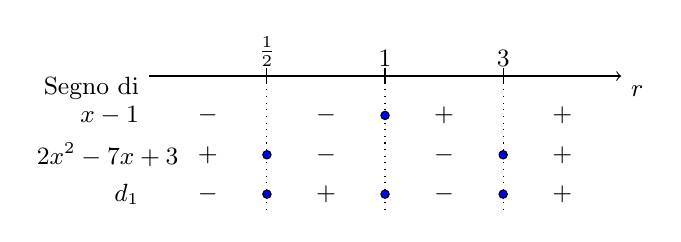
\begin{tikzpicture}[font=\small,x=10mm, y=10mm]

\draw[->] (0,0) -- (6,0) node [below right] () {$r$};

\foreach \x in {1.5,3,4.5}{
\draw(\x,3pt)--(\x,-3pt);
\begin{scope}[dotted]
\draw (\x,0) -- (\x,-1.7);
\end{scope}}

\node[left] at (0,-0.15) {Segno di};
\node[left] at (0,-0.5) {$x-1$};
\node[left] at (.5,-1) {$2x^2-7x+3$};
\node[left] at (0,-1.5) {$d_1$};
\node[above]  at (1.5,0) {$\frac{1}{2}$};
\node[above]  at (3,0) {$1$};
\node[above]  at (4.5,0) {$3$};
\node[] at (.75,-0.5) {$-$};
\node[] at (2.25,-0.5) {$-$};
\node[] at (3.75,-0.5) {$+$};
\node[] at (5.25,-0.5) {$+$};
\node[] at (.75,-1) {$+$};
\node[] at (2.25,-1) {$-$};
\node[] at (3.75,-1) {$-$};
\node[] at (5.25,-1) {$+$};
\node[] at (.75,-1.5) {$-$};
\node[] at (2.25,-1.5) {$+$};
\node[] at (3.75,-1.5) {$-$};
\node[] at (5.25,-1.5) {$+$};

\draw[fill=blue] (3,-.5)circle (1.5pt);
\draw[fill=blue] (1.5,-1)circle (1.5pt);
\draw[fill=blue] (4.5,-1)circle (1.5pt);
\draw[fill=blue] (3,-1.5)circle (1.5pt);
\draw[fill=blue] (1.5,-1.5)circle (1.5pt);
\draw[fill=blue] (4.5,-1.5)circle (1.5pt);

\end{tikzpicture}

% \end{center}
% La disequazione è verificata negli intervalli dove è presente il
% segno ``$+$''.
% \[\IS=\left\{x\in\insR/x<\frac{4}{5}\vee~3<x<\frac{9}{2}\right\}.\]
% \end{esempio}
% 
% \begin{esempio}
% $4x^{3}+4x^{2}\le~1+x.$
% La disequazione è di terzo grado; trasportiamo al primo membro tutti i
% monomi:
% \[4x^{3}+4x^{2}-1-x\le~0.\]
% 
% Possiamo risolverla se riusciamo a scomporre in fattori di primo grado
% il polinomio al primo membro:
% \[4x^{3}+4x^{2}-1-x=4x^{2}(x+1)-(x+1)=(x+1)(4x^2-1) \Rightarrow 
% (x+1)(2x-1)(2x+1)\le~0.\]
% 
% Studiamo ora il segno di ciascun fattore, tenendo conto che sono
% richiesti anche i valori che annullano ogni singolo fattore (legge di
% annullamento del prodotto):
% 
% \[ F_{1}:x+1\ge~0\Rightarrow x\ge -1;\quad F_{2}:2x-1\ge~0\Rightarrow 
% x\ge \dfrac{1}{2},\quad F_{3}:2x+1\ge~0\Rightarrow x\ge -{\dfrac{1}{2}}.\]
% Possiamo ora costruire la tabella dei segni.
% Ricordiamo che la disequazione di partenza~$4x^{3}+4x^{2}\le~1+x$ è
% verificata dove compare il segno~``$-$'':
% 
% \begin{center}
% % (c) 2013 Claudio Carboncini - claudio.carboncini@gmail.com
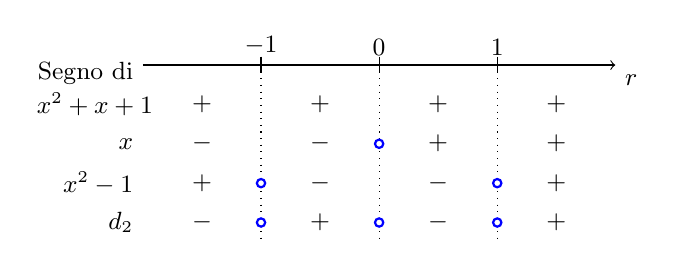
\begin{tikzpicture}[font=\small,x=10mm, y=10mm]

\draw[->] (0,0) -- (6,0) node [below right] () {$r$};

\foreach \x in {1.5,3,4.5}{
\draw(\x,3pt)--(\x,-3pt);
\begin{scope}[dotted]
\draw (\x,0) -- (\x,-2.2);
\end{scope}}

\node[left] at (0,-0.1) {Segno di};
\node[left] at (.25,-0.5) {$x^2+x+1$};
\node[left] at (0,-1) {$x$};
\node[left] at (0,-1.5) {$x^2-1$};
\node[left] at (0,-2) {$d_2$};
\node[above]  at (1.5,0) {$-1$};
\node[above]  at (3,0) {$0$};
\node[above]  at (4.5,0) {$1$};
\node[] at (.75,-0.5) {$+$};
\node[] at (2.25,-0.5) {$+$};
\node[] at (3.75,-0.5) {$+$};
\node[] at (5.25,-0.5) {$+$};
\node[] at (.75,-1) {$-$};
\node[] at (2.25,-1) {$-$};
\node[] at (3.75,-1) {$+$};
\node[] at (5.25,-1) {$+$};
\node[] at (.75,-1.5) {$+$};
\node[] at (2.25,-1.5) {$-$};
\node[] at (3.75,-1.5) {$-$};
\node[] at (5.25,-1.5) {$+$};
\node[] at (.75,-2) {$-$};
\node[] at (2.25,-2) {$+$};
\node[] at (3.75,-2) {$-$};
\node[] at (5.25,-2) {$+$};

\begin{scope}[blue,thick]
\draw[fill=white] (3,-1)circle (1.5pt);
\draw[fill=white] (1.5,-1.5)circle (1.5pt);
\draw[fill=white] (4.5,-1.5)circle (1.5pt);
\draw[fill=white] (3,-2)circle (1.5pt);
\draw[fill=white] (1.5,-2)circle (1.5pt);
\draw[fill=white] (4.5,-2)circle (1.5pt);
\end{scope}

\end{tikzpicture}

% \end{center}
% \[\IS=\left\{x\in \insR/x\le-1\text{ oppure }-\frac{1}{2}\le 
% x\le\frac{1}{2}\right\}.\]
% \end{esempio}
% % \end{exrig}
% 
% \begin{procedura}
%  Determinare l'$\IS$ Di una disequazione polinomiale di grado
% superiore al primo:
% 
% \begin{enumeratea}
%  \item scrivere la disequazione nella forma~$p\leq0$, $p\geq~0$,
% $p<0$, $p>0$
% \item scomporre in fattori irriducibili il polinomio;
% \item determinare il segno di ciascun fattore, ponendolo sempre maggiore
% di zero, o maggiore uguale a zero a seconda della richiesta del
% problema;
% \item costruire la tabella dei segni, segnando con un punto ingrossato
% gli zeri del polinomio;
% \item determinare gli intervalli in cui il polinomio assume il segno
% richiesto.
% \end{enumeratea}
% \end{procedura}
% 
% % \ovalbox{\risolvii \ref{ese:21.44}, \ref{ese:21.45}, \ref{ese:21.46}, 
% % \ref{ese:21.47}, \ref{ese:21.48}, \ref{ese:21.49}, \ref{ese:21.50}, 
% % \ref{ese:21.51},
% % \ref{ese:21.52}, \ref{ese:21.53}}
% 
% \section{Disequazioni frazionarie}
% \label{sec:compl1_disequazionifratte}
% 
% Un'espressione contenente operazioni tra frazioni
% algebriche ha come risultato una frazione algebrica. Con la condizione
% di esistenza che il denominatore della frazione sia diverso da zero la
% ricerca del segno di una frazione algebrica viene effettuata con la
% stessa procedura seguita per il prodotto di due o più fattori.
% 
% % \begin{exrig}
%  \begin{esempio}
%  $p=\dfrac{3x-7}{2-x}\ge~0$.
% 
%  Poniamo innanzi tutto la~$\CE: 2-x\neq~0$
%  cioè~$x\neq~2$ e procediamo studiando il segno del
% numeratore e del denominatore. Terremo conto della~$\CE$ ponendo il
% denominatore semplicemente maggiore di zero e non maggiore uguale.
% \[N\ge~0\Rightarrow~3x-7\ge~0\Rightarrow x\ge \frac{7}{3},\]
% \[D>0\Rightarrow2-x>0\Rightarrow \ x<2.\]
% \begin{center}
% % (c) 2012 Dimitrios Vrettos - d.vrettos@gmail.com
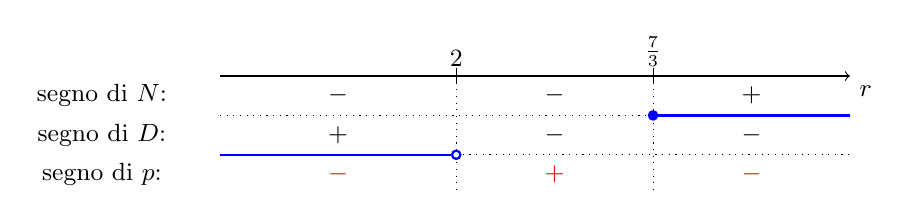
\begin{tikzpicture}[font=\small,x=10mm, y=10mm]

\draw[->] (0,0) -- (8,0) node [below right] () {$r$};

\foreach \x in {3,5.5}{
\draw(\x,3pt)--(\x,-3pt);
\begin{scope}[dotted]
\draw (\x,0) -- (\x,-1.5);
\draw (0,-.5) -- (5.5,-.5);
\draw (3,-1) -- (8,-1);
\end{scope}}

\node[above]  at (3,0) {$2$};
\node[above]  at (5.5,0) {$\frac{7}{3}$};

\begin{scope}[blue,thick]
\draw (5.5,-.5) -- (8,-.5);
\draw (3,-1) -- (0,-1);

\draw[fill=blue] (5.5,-.5)circle (1.5pt);
\draw[fill=white] (3,-1)circle (1.5pt);
\end{scope}

\foreach \x in {-1.5}{
\node  at (\x,-.25) {segno di $N$:};
\node  at (\x,-.75) {segno di $D$:};
\node  at (\x,-1.25) {segno di $p$:};
}
\foreach \z in {1.5,4.25}
\node  at (\z,-.25) {$-$};

\foreach \zi in {4.25,6.75}
\node  at (\zi,-.75) {$-$};

\node  at (6.75,-.25) {$+$};
\node  at (1.5,-.75) {$+$};

\begin{scope}[red]
\foreach \y in {-1.25}{
\foreach \ziv in {4.25}
	\node at (\ziv,\y) {$+$};
\foreach \zv in {1.5,6.75}
\node at (\zv,\y) {$-$};
}
\end{scope}
\end{tikzpicture}
% \end{center}
% Analogamente a quanto fatto per il prodotto, dalla tabella dei segni otteniamo
% \[\IS=\left\{x\in \insR/2<x\le \frac{7}{3}\right\}\]
% in cui vediamo già compresa la~$\CE$ che inizialmente avevamo posto.
%  \end{esempio}
% % \end{exrig}
% 
% \begin{procedura}
%  Procedura per determinare~$\IS$ di una disequazione frazionaria:
% 
% \begin{enumeratea}
%  \item applicare il primo principio e trasportare tutti i termini al primo 
%   membro;
%  \item eseguire i calcoli dell'espressione al primo membro per arrivare a una 
%   disequazione nella forma:
%  \subitem $\dfrac{N(x)}{D(x)}>0$ oppure~$\dfrac{N(x)}{D(x)}\ge~0$ 
%   oppure~$\dfrac{N(x)}{D(x)}<0$ oppure~$\dfrac{N(x)}{D(x)}\le~0$
%  \item studiare il segno del numeratore e del denominatore, ponendo~$N(x)>0$ 
%   (oppure~$N(x)\geq~0$ a secondo della richiesta) e~$D(x)>0$
%  \item costruire la tabella dei segni, segnando con un punto in grassetto gli 
%   zeri del numeratore;
%  \item determinare gli intervalli in cui il polinomio assume il segno 
%   richiesto.
% \end{enumeratea}
% \end{procedura}
% 
% % \begin{exrig}
%  \begin{esempio}
%  $\dfrac{x-1}{2x+2}+\dfrac{2x+1}{4x-2}>
%  \dfrac{4x^{2}(2x+1)+1}{8x^{3}+8x^{2}-2x-2}.$
% 
% Trasportiamo tutti i termini al primo 
% membro~$\dfrac{x-1}{2x+2}+\dfrac{2x+1}{4x-2}-
%         \dfrac{4x^{2}(2x+1)+1}{8x^{3}+8x^{2}-2x-2}>0$.
% 
% Scomponiamo in fattori i denominatori, determiniamo il minimo comune
% multiplo e sommiamo le frazioni per arrivare alla forma~$\frac{N(x)}{D(x)}>0$:
% 
% \begin{align}
% &\frac{x-1}{2(x+1)}+\frac{2x+1}{2(2x-1)}-
%  \frac{4x^{2}(2x+1)+1}{2(x+1)(2x-1)(2x+1)}>0 \notag\\
% \Rightarrow & \frac{(x-1)(2x-1)(2x+1)+(2x+1)(2x+1)(x+1)-
%  4x^{2}(2x+1)+1}{2(x+1)(2x-1)(2x+1)}>0 \notag\\
% \Rightarrow & \frac{4x+1}{2(x+1)(2x-1)(2x+1)}>0. \label{eq:21.1}
% \end{align}
% Studiamo separatamente il segno di tutti i fattori che compaiono nella
% frazione, sia quelli al numeratore sia quelli al denominatore e
% costruiamo la tabella dei segni:
%  \[\begin{gathered}
%  N>0\Rightarrow~4x+1>0\Rightarrow x>-{\frac{1}{4}},\\
%  D>0\Rightarrow\left\{\begin{array}{l}
%   x+1>0\Rightarrow x>-1 \\
%   2x-1>0\Rightarrow x>\frac{1}{2}\\
%   2x+1>0\Rightarrow x>-{\frac{1}{2}}
% \end{array}\right..
% \end{gathered}\]
% \begin{center}
% % (c) 2012 Dimitrios Vrettos - d.vrettos@gmail.com
\begin{tikzpicture}[font=\small,x=10mm, y=10mm]

  \draw[->] (0,0) -- (8,0) node [below right] () {$r$};

  \foreach \x in {1.5,2.75,3.75,5.75}{
    \draw(\x,3pt)--(\x,-3pt);
    
    \begin{scope}[dotted]
      \draw (\x,0) -- (\x,-2.5);
      \draw (0,-.5) -- (3.75,-.5);
      \draw (0,-1) -- (1.5,-1);
      \draw (0,-1.5) -- (5.75,-1.5);
      \draw (0,-2) -- (2.75,-2);
    \end{scope}
  }

  \node[above]  at (1.5,0) {$-1$};
  \node[above] at (2.75,0) {$-\frac{1}{2}$};
  \node[above]  at (3.75,0) {$-\frac{1}{4}$};
  \node[above]  at (5.75,0) {$\frac{1}{2}$};

  \begin{scope}[blue,thick]
    \draw (3.75,-.5) -- (8,-.5);
    \draw (1.5,-1) -- (8,-1);
    \draw (5.75,-1.5) -- (8,-1.5);
    \draw (2.75,-2) -- (8,-2);

    \draw[fill=white] (3.75,-.5)circle (1.5pt);
    \draw[fill=white] (1.5,-1)circle (1.5pt);
    \draw[fill=white] (5.75,-1.5)circle (1.5pt);
    \draw[fill=white] (2.75,-2)circle (1.5pt);
  \end{scope}

  \foreach \x in {-1.5}{
    \node  at (\x,-.25) {segno di $N$:};
    \node(d1)  at (\x,-.75) {segno di $d_1$:};
    \node  at (\x,-1.25) {segno di $d_2$:};
    \node (d3) at (\x,-1.75) {segno di $d_3$:};
    \node  at (\x,-2.25) {segno di $f$:};
    }

  \draw[decorate, decoration={brace, mirror}] let \p1=(d1.north west), \p2=(d3.south west) in(\p1 ) -- (\p2) node[midway, left=2pt] {$D:$};

  \foreach \z in {.75, 2.125,3.25}
    \node  at (\z,-.25) {$-$};

  \foreach \zi in {4.75, 6.875}
    \node  at (\zi,-.25) {$+$};

  \foreach \zii in {2.125,3.25,4.75, 6.875}
    \node  at (\zii,-.75) {$+$};

  \foreach \ziii in {.75,2.125,3.25,4.75}
    \node  at (\ziii,-1.25) {$-$};

  \foreach \ziv in {.75,2.125}
    \node at (\ziv,-1.75) {$-$};

  \foreach \zv in {3.25,4.75, 6.875}
    \node at (\zv,-1.75) {$+$};

  \node  at (.75,-.75) {$-$};
  \node  at (6.875,-1.25) {$+$};

  \begin{scope}[red]
    \foreach \y in {-2.25}{
      \foreach \ziv in {.75,3.25,6.875}
	\node at (\ziv,\y) {$+$};
      \foreach \zv in {2.125,4.75}
	\node at (\zv,\y) {$-$};
    }
  \end{scope}
\end{tikzpicture}
% \end{center}
% Non abbiamo posto le~$\CE$ in quanto già rispettate dalle disequazioni
% del denominatore.
% Prendiamo gli intervalli in cui il segno della frazione è positivo
% come richiesto dalla disequazione~\ref{eq:21.1}:
%  \[\IS=\left\{x\in \insR/x<-1\vee -{\frac{1}{2}}<x<-{\frac{1}{4}}\vee 
%  x>\frac{1}{2}\right\}.\]
% \end{esempio}
% 
%  \begin{esempio}
% $\dfrac{x}{2}-\dfrac{2}{3}\cdot {\dfrac{2x-3}{x-1}}+\dfrac{10x-3}{6x-6}\le
% \dfrac{3}{2}\cdot {\dfrac{x^{2}+2}{3x-2}}+\dfrac{1}{3(x-1)(3x-2)}.$
% 
% Trasportiamo tutti i termini al primo membro:
% \[\frac{x}{2}-\frac{2}{3}\cdot\frac{2x-3}{x-1}+\frac{10x-3}{6x-6}-
% \frac{3}{2}\cdot\frac{x^{2}+2}{3x-2}-\frac{1}{3(x-1)(3x-2)}\le~0.\]
% 
% Eseguiamo le operazioni per semplificare la frazione e ridurla alla
% forma~$\frac{N(x)}{D(x)}\le~0$:
% 
% \begin{align}
%   &\frac{x}{2}-\frac{4x-6}{3(x-1)}+\frac{10x-3}{6(x-1)}-
%    \frac{3x^{2}+6}{2(3x-2)}-\frac{1}{3(x-1)(3x-2)}\le~0\notag\\
%   \Rightarrow &\frac{3x(x-1)(3x-2)-2(4x-6)(3x-2)+(10x-3)(3x-2)-
%   3(3x^{2}+6)(x-1)-2}{6(x-1)(3x-2)}\le~0\notag\\
%   \Rightarrow &\frac{11x-2}{6(x-1)(3x-2)}\le~0. \label{eq:22.2}
% \end{align}
% 
% Studiamo il segno del numeratore e dei fattori del denominatore:
%  \[\begin{gathered}N\ge~0\Rightarrow~11x-2\ge~0\Rightarrow x\ge\frac{2}{11},\\
%   D>0\Rightarrow\left\{\begin{array}{l}
%   d_{1}>0\Rightarrow x-1>0\Rightarrow x>1\\
%   d_{2}>0\Rightarrow~3x-2>0\Rightarrow x>\dfrac{2}{3}
% \end{array}\right.. \end{gathered}\]
% \begin{center}
% % (c) 2012 Dimitrios Vrettos - d.vrettos@gmail.com
\begin{tikzpicture}[font=\small,x=10mm, y=10mm]

\draw[->] (0,0) -- (8,0) node [below right] () {$r$};

\foreach \x in {1,3.72,5.56}{
\draw(\x,3pt)--(\x,-3pt);
\begin{scope}[dotted]
\draw (\x,0) -- (\x,-2);
\draw (0,-.5) -- (1,-.5);
\draw (0,-1) -- (5.56,-1);
\draw (0,-1.5) -- (3.72,-1.5);

\end{scope}}


\node[above] at (1,0) {$\frac{2}{11}$};
\node[above]  at (3.72,0) {$\frac{2}{3}$};
\node[above]  at (5.56,0) {$1$};

\begin{scope}[blue,thick]
\draw (1,-.5) -- (8,-.5);
\draw (5.56,-1) -- (8,-1);
\draw (3.72,-1.5) -- (8,-1.5);

\draw[fill=blue] (1,-.5)circle (1.5pt);
\draw[fill=white] (5.56,-1)circle (1.5pt);
\draw[fill=white] (3.72,-1.5)circle (1.5pt);
\end{scope}

\foreach \x in {-1.5}{
\node  at (\x,-.25) {segno di $N$:};
\node(d1)  at (\x,-.75) {segno di $d_1$:};
\node (d2) at (\x,-1.25) {segno di $d_2$:};
\node (d3) at (\x,-1.75) {segno di $f$:};
}

 \draw[decorate, decoration={brace, mirror}]  let \p1=(d1.north west), \p2=(d2.south west) in(\p1 ) -- (\p2) node[midway, left=2pt] {$D:$};

\foreach \z in {2.36,4.64,6.78}
\node  at (\z,-.25) {$+$};

 \foreach \zi in {.5,2.36,4.64}
 \node  at (\zi,-.75) {$-$};

\foreach \zii in {.5,2.36}
 \node  at (\zii,-1.25) {$-$};

 \foreach \ziii in {4.64,6.78}
\node  at (\ziii,-1.25) {$+$};

\node  at (.5,-.25) {$-$};
\node  at (6.78,-.75) {$+$};

\begin{scope}[red]
\foreach \y in {-1.75}{
\foreach \ziv in {.5,4.64}
	\node at (\ziv,\y) {$-$};
\foreach \zv in {2.36,6.78}
\node at (\zv,\y) {$+$};
}
\end{scope}
\end{tikzpicture}
% \end{center}
% Non abbiamo posto le~$\CE$ in quanto già rispettate dalle disequazioni
% del denominatore. Prendiamo gli intervalli in cui il segno della frazione è 
% positivo o
% nullo come dalla disequazione~\ref{eq:22.2}:
% \[\IS=\left\{x\in \insR/x\le\frac{2}{11}\vee \frac{2}{3}<x<1\right\}.\]
%  \end{esempio}
% % \end{exrig}
% % \ovalbox{\risolvii \ref{ese:21.54}, \ref{ese:21.55}, \ref{ese:21.56}, 
% \ref{ese:21.57}, \ref{ese:21.58}, \ref{ese:21.59}, \ref{ese:21.60}, 
% \ref{ese:21.61}, \ref{ese:21.62}, \ref{ese:21.63}}
% % 
% % \vspazio\ovalbox{\ref{ese:21.64}, \ref{ese:21.65}, \ref{ese:21.66}, 
% \ref{ese:21.67}, \ref{ese:21.68}, \ref{ese:21.69}}
% % 
% % \cleardoublepage
